\begin{chapter}{Applications and Numerical Experiments}
\label{ch:numericalexperiments}
In the first part of the chapter we apply the algorithms to a variety of problems in image processing, computer vision, medical imaging and related fields.
The second part will be a comparison of the performance of the two implemented minimizer and close with with an numerical experiment investigating the 
dependence of the solution on the changes in the original picture. This is a first step in extending the IRLS algorithm towards recursive splitting into subdomain.\\

As briefly mentioned in the previous section, the test platform is a linux machine with two hyperthreaded 2.8GHz cores Intel i5-2520 (thus a total of four hardware threads)
with AVX vector extensions and 8 GB RAM. 


\section{Image denoising} % (fold)
\label{sec:image denoising}
The very basic application of the algorithm is of course denoising of common 2D grayscale or color pictures.
For grayscale pictures the TV minimization is performed over the Euclidian manifold $M=\mathbb{R}$, while for color
picture, as already explained in the introduction, we have either $M=\mathbb{R}^3$ for the linear-vectorial model or
$M=S^2\times\mathbb{R}$ for the non-linear chromaticity-brightness model.

\subsection{Grayscale} % (fold)
As introductory example  and for the sake of completeness, we show in Figure \ref{fig:application_gray} results from denoising a grayscale image.
\label{sub:Grayscale}
\begin{figure}[h!]
    \centering
    \subfloat[][Original]{
	\label{fig:application_gray_orig}
	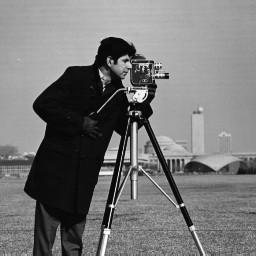
\includegraphics[width=0.325\linewidth]{./figures/experiments/Cameraman.jpg}
    }
    \subfloat[][Noisy]{
	\label{fig:application_gray_noise}
	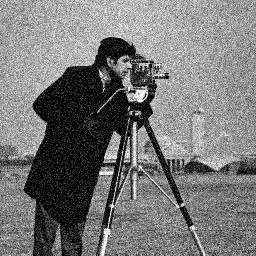
\includegraphics[width=0.325\linewidth]{./figures/experiments/noisy_Cameraman.jpg}
    }
    \subfloat[][Denoised]{
	\label{fig:application_gray_denoised}
	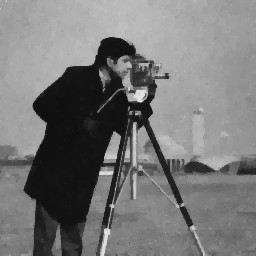
\includegraphics[width=0.325\linewidth]{./figures/experiments/denoised_Cameraman.jpg}
    }\\
    \caption[Color image "Cameraman" grayscale denoising]{Denoising of a grayscale image taking values in the manifold $\mathbb{R}$
	\subref{fig:application_color1_orig} Original image "Lena.jpg", $256\times 256$ px, 8 bit depth
	\subref{fig:application_color1_noise} Componentwise gaussian noise $\mu=0$, $\sigma=0.01$ added
	\subref{fig:application_color1_denoised} Denoised, IRLS with $\lambda=0.09$, $5$ IRLS steps, $1$ newton steps per IRLS step
	\label{fig:application_gray}
    }
\end{figure}
% subsection Grayscale (end)

\FloatBarrier
\subsection{Color} % (fold)
\label{sub:Color}
In this example we perform the TV minimization of color images using the two different color models. In Figure \ref{fig:application_color1}
the among the image processing community well-known \emph{Lena} picture, which is rather small in size. Minimization in
the linear-vectorial color model using 5 IRLS iterations with one Newton step per reweighting is completed within $XXX$ seconds.\\

% subsection Color (end)
\begin{figure}[h!]
    \centering
    \subfloat[][Original]{
	\label{fig:application_color1_orig}
	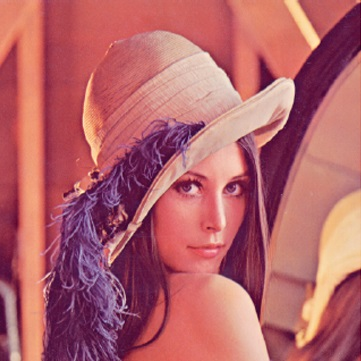
\includegraphics[width=0.325\linewidth]{./figures/experiments/Lena.jpg}
    }
    \subfloat[][Noisy]{
	\label{fig:application_color1_noise}
	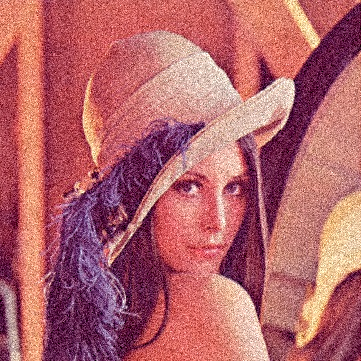
\includegraphics[width=0.325\linewidth]{./figures/experiments/Lena_noise.jpg}
    }
    \subfloat[][Denoised]{
	\label{fig:application_color1_denoised}
	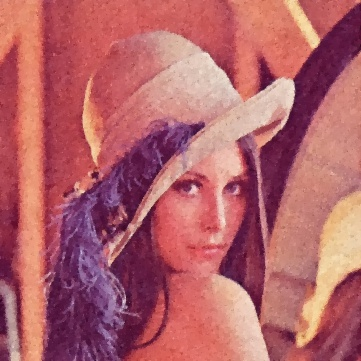
\includegraphics[width=0.325\linewidth]{./figures/experiments/denoised_Lena_noise.jpg}
    }\\
    \caption[Color image "Lena" linear vectorial denoising]{Denoising of a color images using the linear vectorial color model which corresponds to the manifold $\mathbb{R}^3$
	\subref{fig:application_color1_orig} Original image "Lena.jpg", $361\times 361$ px, 8 bit color depth
	\subref{fig:application_color1_noise} Componentwise gaussian noise $\mu=0$, $\sigma=?$ added
	\subref{fig:application_color1_denoised} Denoised, IRLS with $\lambda=?$, $5$ IRLS steps, $1$ newton steps per IRLS step
	\label{fig:application_color1}
    }
\end{figure}

Next, using the same model and parameters we denoise a different image with a size already in the megapixel range. The needed
time, however, is with $XXX$ seconds quite high. The result can be seen in Figure \ref{fig:application_color2}.\\

\begin{figure}[h!]
    \centering
    \subfloat[][Original]{
	\label{fig:application_color2_orig}
	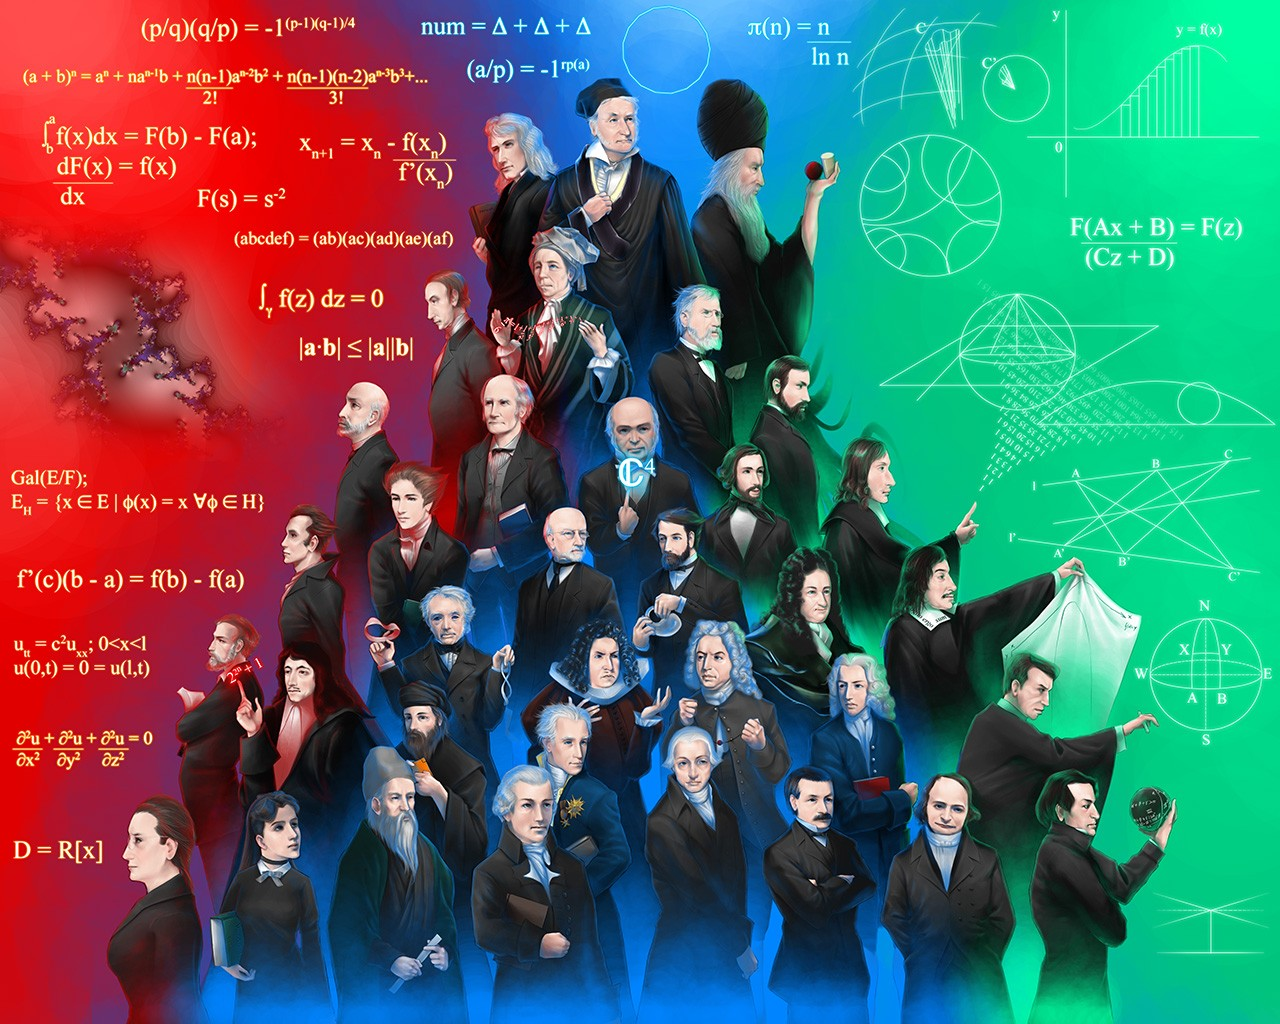
\includegraphics[width=0.325\linewidth]{./figures/experiments/mathematicians.jpg}
    }
    \subfloat[][Noisy]{
	\label{fig:application_color2_noise}
	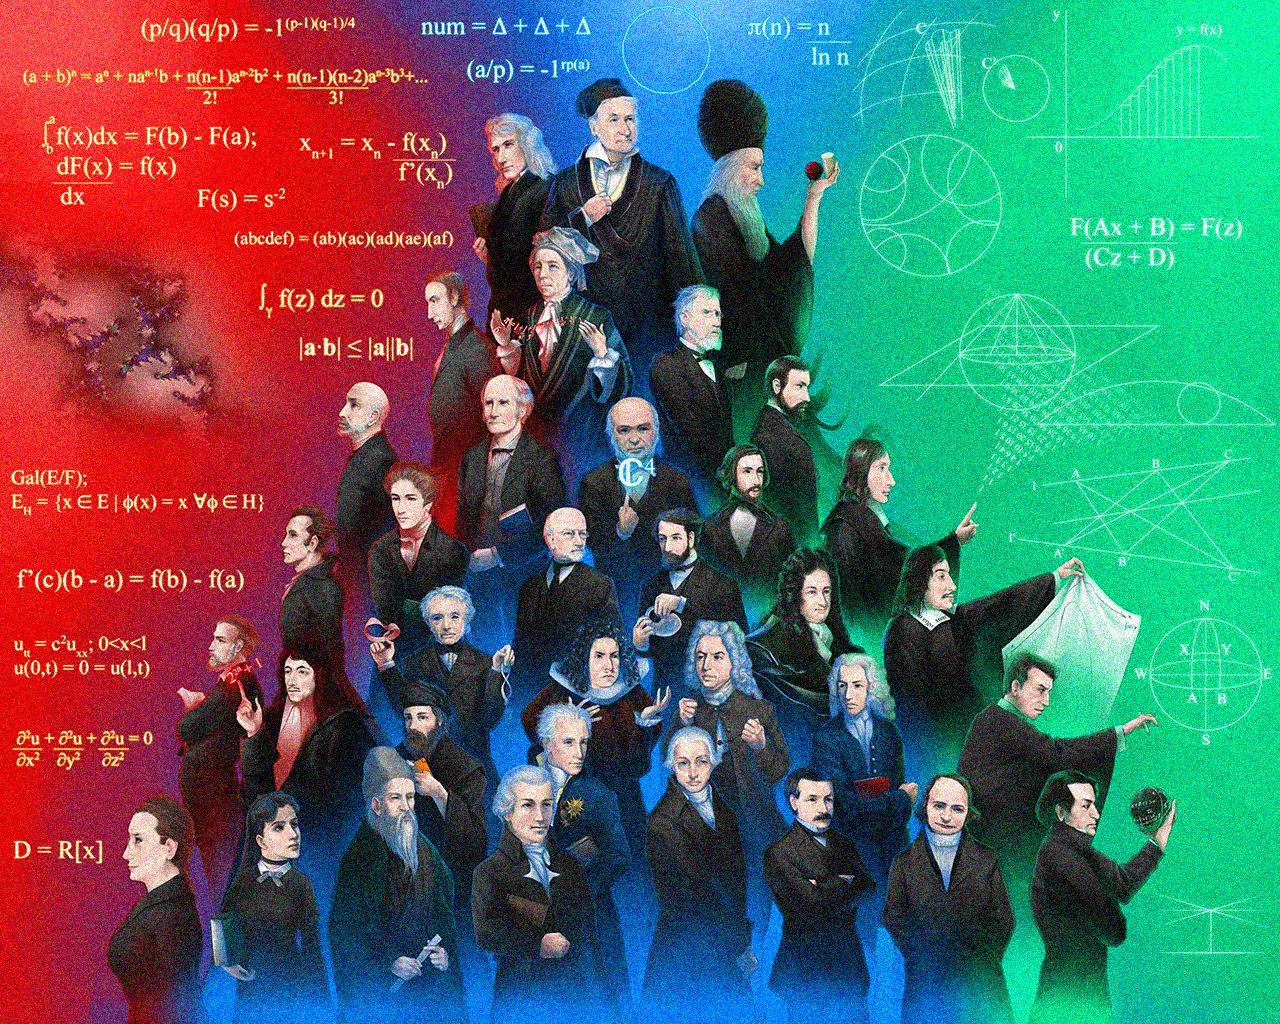
\includegraphics[width=0.325\linewidth]{./figures/experiments/noisy_mathematicians.jpg}
    }
    \subfloat[][Denoised]{
	\label{fig:application_color2_denoised}
	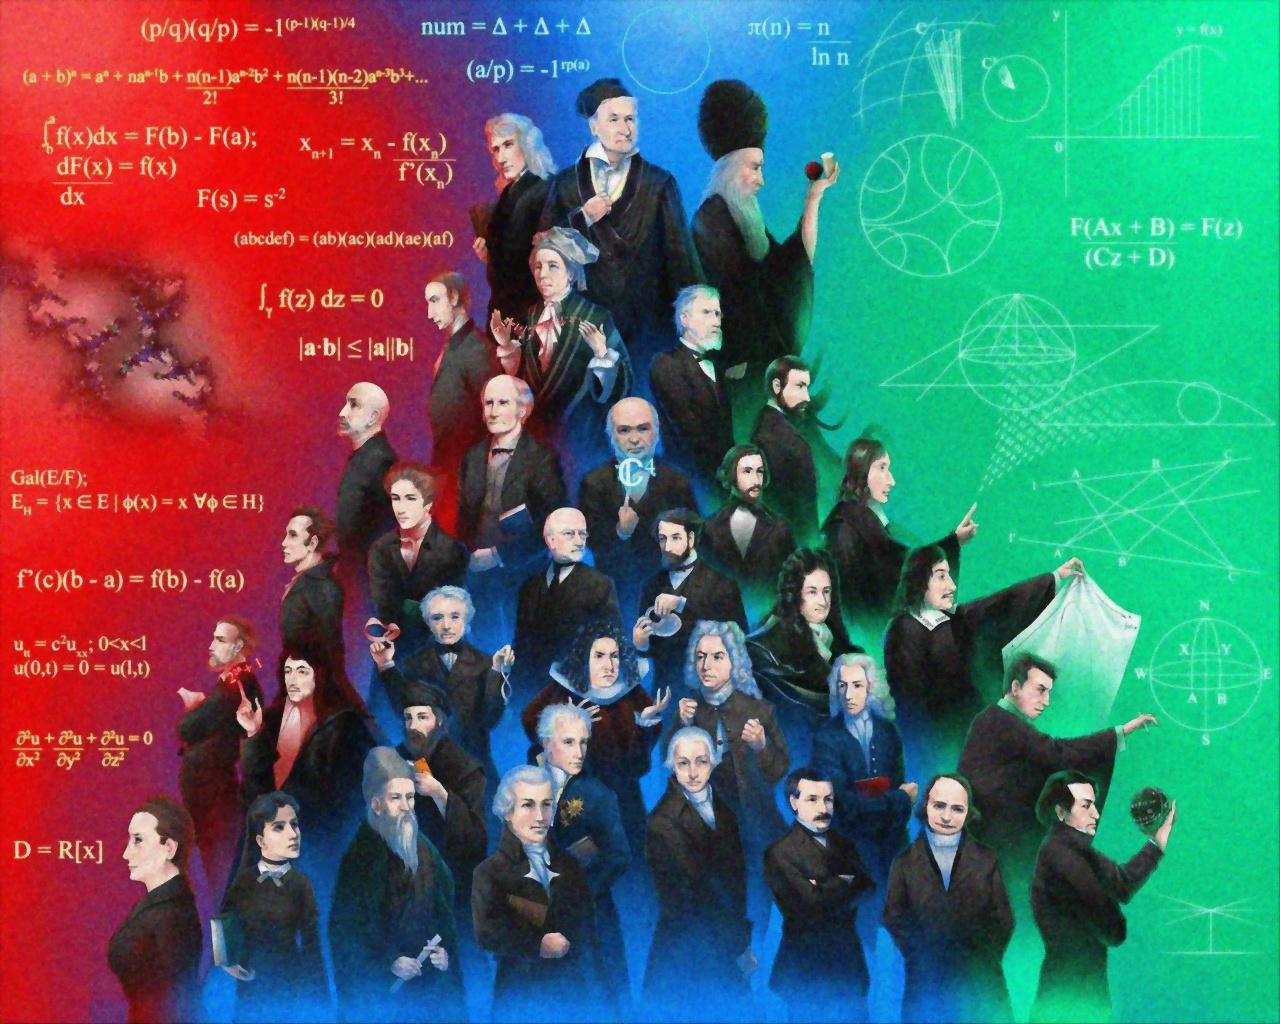
\includegraphics[width=0.325\linewidth]{./figures/experiments/denoised_noisy_mathematicians.jpg}
    }\\
    \caption[Large image "mathematicians" linear-vectorial denoising]{Denoising of a color images using the linear vectorial color model which corresponds to the manifold $\mathbb{R}^3$
	\subref{fig:application_color2_orig} Original image "mathematicians.jpg", $1280\times 1024$ px, 8 bit color depth
	\subref{fig:application_color2_noise} Componentwise gaussian noise $\mu=0$, $\sigma=?$ added
	\subref{fig:application_color2_denoised} Denoised, IRLS with $\lambda=?$, $?$ IRLS steps, $?$ newton steps per IRLS step
	\label{fig:application_color2}
    }
\end{figure}

Finally, in Figure \ref{fig:application_color3} we denoise a third picture using the chromaticity-brightness model. Here minimization over the product manifold
$S^2\times \mathbb{R}$ is performed by denoising the chromaticity($S^2$) and the brightness($\mathbb{R}$) separately, which has the added advantage of more 
fine-grained control over the process because two $\lambda$ parameters can be chosen separately for each part, too.

\begin{figure}[h!]
    \centering
    \subfloat[][Original]{
	\label{fig:application_color3_orig}
	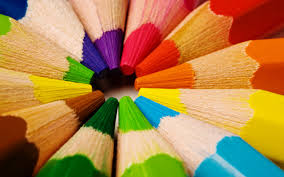
\includegraphics[width=0.325\linewidth]{./figures/experiments/crayons.jpg}
    }
    \subfloat[][Noisy]{
	\label{fig:application_color3_noise}
	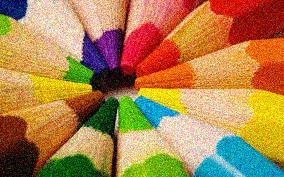
\includegraphics[width=0.325\linewidth]{./figures/experiments/noisy_crayons.jpg}
    }
    \subfloat[][Denoised]{
	\label{fig:application_color3_denoised}
	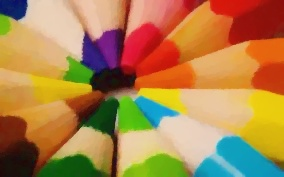
\includegraphics[width=0.325\linewidth]{./figures/experiments/denoised(CBR)_noisy_crayons.jpg}
    }\\
    \caption[Large image "crayons" CBR-vectorial denoising]{Denoising of a color images using the linear vectorial color model which corresponds to the manifold $S^2\times\mathbb{R}$
	\subref{fig:application_color3_orig} Original image "mathematicians.jpg", $284\times 177$ px, 8 bit color depth
	\subref{fig:application_color3_noise} Componentwise gaussian noise $\mu=0$, $\sigma=?$ added
	\subref{fig:application_color3_denoised} Denoised, IRLS with $\lambda_{\mathbb{R}}=0.1$, $5$ IRLS steps, $1$ newton steps per IRLS step
	\label{fig:application_color3}
    }
\end{figure}

\FloatBarrier
\subsection{Inpainting} % (fold)
We consider a damaged picture were a considerable part of the picture has been overpainted with blue color. In the first step we detect the damaged region which in this
case is done via a simple color selector (e.g. all pixels with a blue value larger than 0.95). In principle many other selection methods known from common raster graphic editors
could be implemented here as well. \\
Next, the a first guess is calculated using scattered linear interpolation and lastly the TV minimization itself is performed. The process is summarized in Figure 
\ref{fig:application_colorinpaint1}.

\label{sub:Inpainting}
\begin{figure}[h!]
    \centering
    \subfloat[][Original]{
	\label{fig:application_colorinpaint1_orig}
	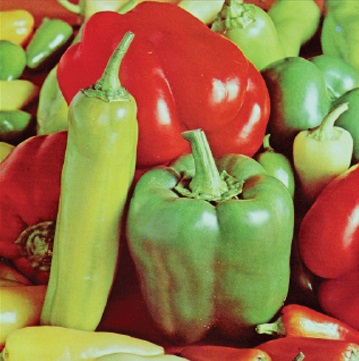
\includegraphics[width=0.25\linewidth]{./figures/experiments/Pepper.jpg}
    }
    \subfloat[][Damaged]{
	\label{fig:application_colorinpaint1_dam}
	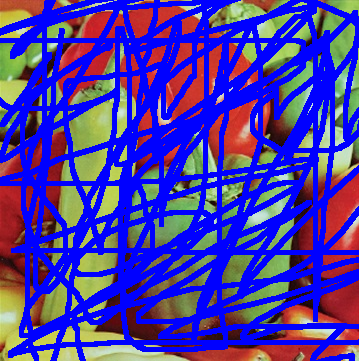
\includegraphics[width=0.25\linewidth]{./figures/experiments/Pepper_dam.png}
    }
    \subfloat[][First guess]{
	\label{fig:application_colorinpaint1_guess}
	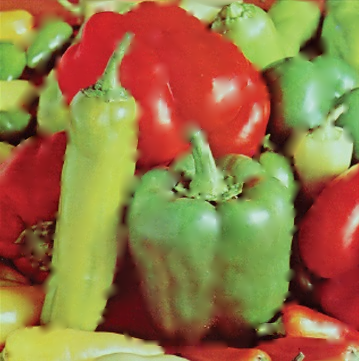
\includegraphics[width=0.25\linewidth]{./figures/experiments/firstguess_Pepper_dam.png}
    }
    \subfloat[][Restored]{
	\label{fig:application_colorinpaint1_restored}
	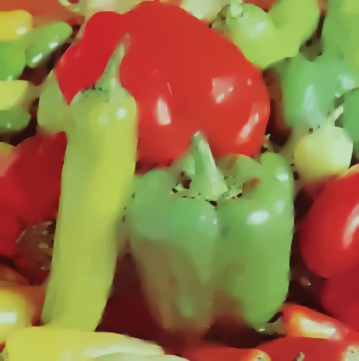
\includegraphics[width=0.25\linewidth]{./figures/experiments/denoised_Pepper_dam.png}
    }\\
    \caption[Denoising linear vectorial]{Denoising of a color images using the linear vectorial color model which corresponds to the manifold $\mathbb{R}^3$
	\subref{fig:application_colorinpaint1_orig} Original image "Pepper.png", $359\times 361$ px, 8 bit color depth
	\subref{fig:application_colorinpaint1_dam} Damaged by overpainting with blue color
	\subref{fig:application_colorinpaint1_guess} First guess via componentwise scattered interpolation
	\subref{fig:application_colorinpaint1_restored} Restored, IRLS with $\lambda=?$, $?$ IRLS steps, $?$ newton steps per IRLS step
	\label{fig:application_colorinpaint1}
    }
\end{figure}

% subsection Inpainting (end)


\FloatBarrier
\subsection{Recolorization} % (fold)
\label{sub:Recolorization}
Colarization, also known is color inpainting, because it is basically just a special of inpainting is performed in the next example.
Here the picture is not necessarily noisy but we assume only the brightness of each pixel is known, while the chromaticity is known only for a low ratio $r=0.01$ of all pixels.
Note that this splitting implies that inpainting and TV minimization takes place only $S^2$.\\

As in the previous example, we first have to detect all damaged, i.e. non-colored, pixels to inpaint. Again we use scattered interpolation to obtain the first guess which is depcited
in Figure \ref{fig:application_colorinpaint1} \subref{fig:application_colorinpaint1_guess}. One can observe that the color runs over the edges of leafes. To avoid this we need to
detect the edges in the brightness part using the Canny edge detector \cite{Canny}, for example, and set the edge weights for the chromaticity part accordingly. As a result, we indeed
obtain sharp and clear edges in the final result \ref{fig:application_colorinpaint1} \subref{fig:application_colorinpaint1_restored}.

\begin{figure}[h!]
    \centering
    \subfloat[][Original]{
	\label{fig:application_colorization1_orig}
	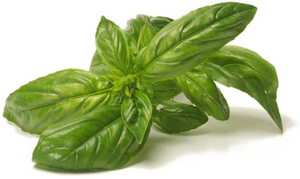
\includegraphics[width=0.25\linewidth]{./figures/experiments/Basil.jpg}
    }
    \subfloat[][Colors removed]{
	\label{fig:application_colorization1_colorless}
	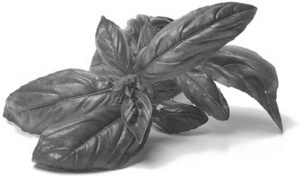
\includegraphics[width=0.25\linewidth]{./figures/experiments/colorless_Basil.jpg}
    }
    \subfloat[][First guess]{
	\label{fig:application_colorization1_guess}
	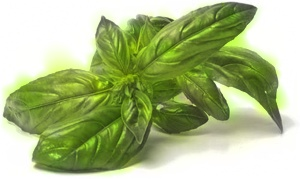
\includegraphics[width=0.25\linewidth]{./figures/experiments/recolored_fg_Basil.jpg}
    }
    \subfloat[][Recolored]{
	\label{fig:application_colorization1_restored}
	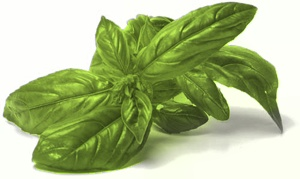
\includegraphics[width=0.25\linewidth]{./figures/experiments/recolored_Basil.jpg}
    }\\
    \caption[Recolorization]{Recolorization using color inpainting in the Chromaticity-Brightness color model, corresponding to $S^2\times\mathbb{R}$
	\subref{fig:application_colorization1_orig} Original image "Basil.jpg", $300\times 179$ px, 8 bit color depth
	\subref{fig:application_colorization1_colorless} Image with a ratio of approximately $0.01$ remaining colored pixels
	\subref{fig:application_colorization1_guess} First guess via componentwise scattered interpolation
	\subref{fig:application_colorization1_restored} Recolored, IRLS with $\lambda=?$, $?$ IRLS steps, $?$ newton steps per IRLS step
	\label{fig:application_colorization1}
    }
\end{figure}
% subsection Recolorization (end)

\FloatBarrier
\subsection{Volume images} % (fold)
\label{sub:Volume images}
We conclude the picture section with an example of a 3D volume image as they might occur in medical imaging from magnetic resonance imaging (MRI) or
computed tomography. In this demonstration, however, we chose the example of the so-called \emph{Boston teapot}, taken a volume image library \cite{volumeLib}
and added componentwise gaussian noise. The image represents only intensity values, hence minimization is performed over $\mathbb{R}$. The result are shown
in Figure \ref{fig:application_volume1_orig}.\\

For this picture we used the proximal point algorithm, because the memory and computational requirements of the IRLS for a picture of this size are very high:
In section \label{sub:NewtonequationfortheTVfunctional} it was shown that the dimension of the sparse linear system is $\operatorname{dim}(M)XYZ$ which
in this case amounts to $1.1\times 10^{7}$, which is the length of the gradient while the Hessian will contain $7.7\times 10^{7}$ non-zero-entries.
The solution of a sparse linear system of that size is computationally very demanding while in comparison the geodesic averaging and karcher mean calculations
simplify to mostly vectorized addition and subtraction operations on a simple manifold like $\mathbb{R}$.

\begin{figure}[h!]
    \centering
    \subfloat[][Original]{
	\label{fig:application_volume1_orig}
	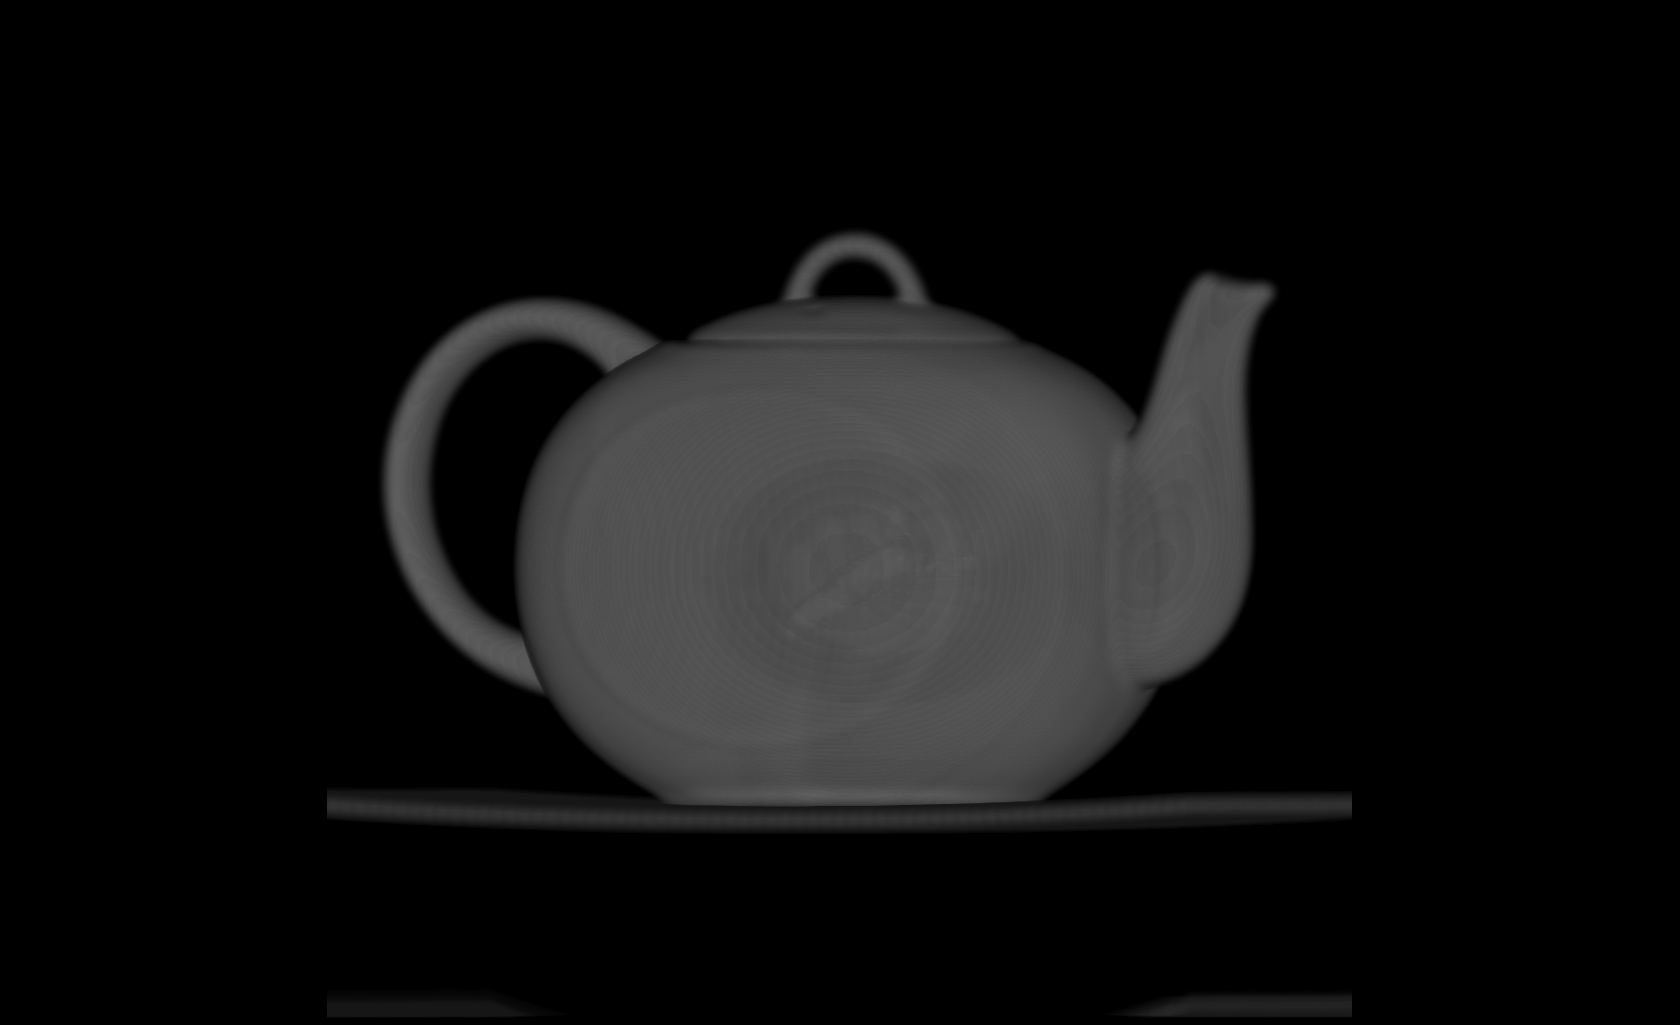
\includegraphics[width=0.325\linewidth]{./figures/experiments/VolumeImg.png}
    }
    \subfloat[][Noisy]{
	\label{fig:application_volume1_noise}
	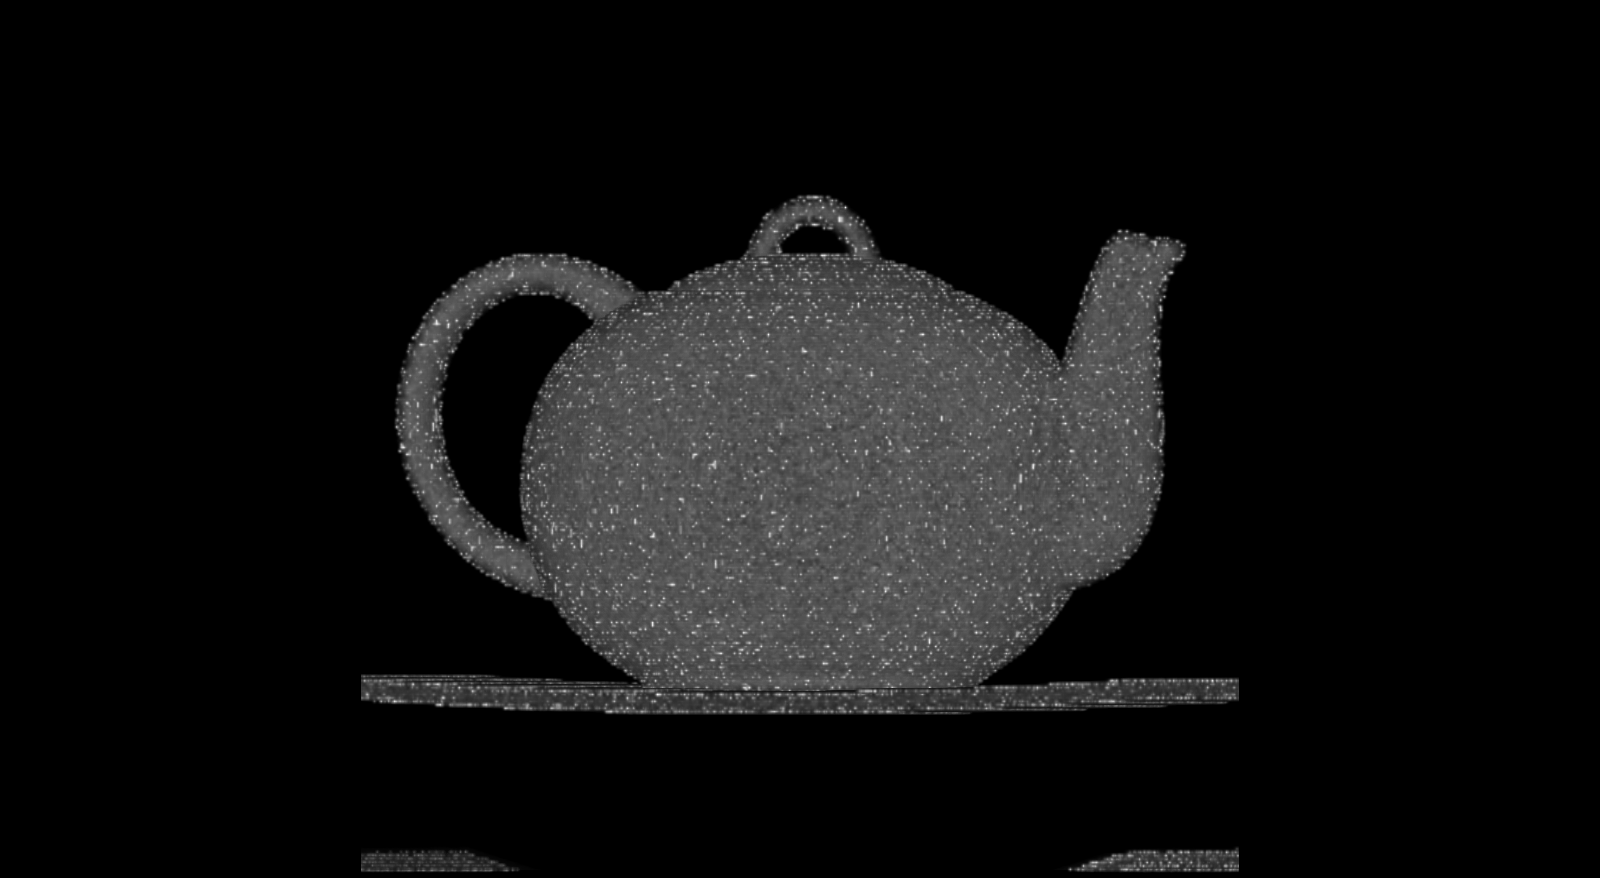
\includegraphics[width=0.325\linewidth]{./figures/experiments/noisyVolumeImg.png}
    }
    \subfloat[][Denoised]{
	\label{fig:application_volume1_denoised}
	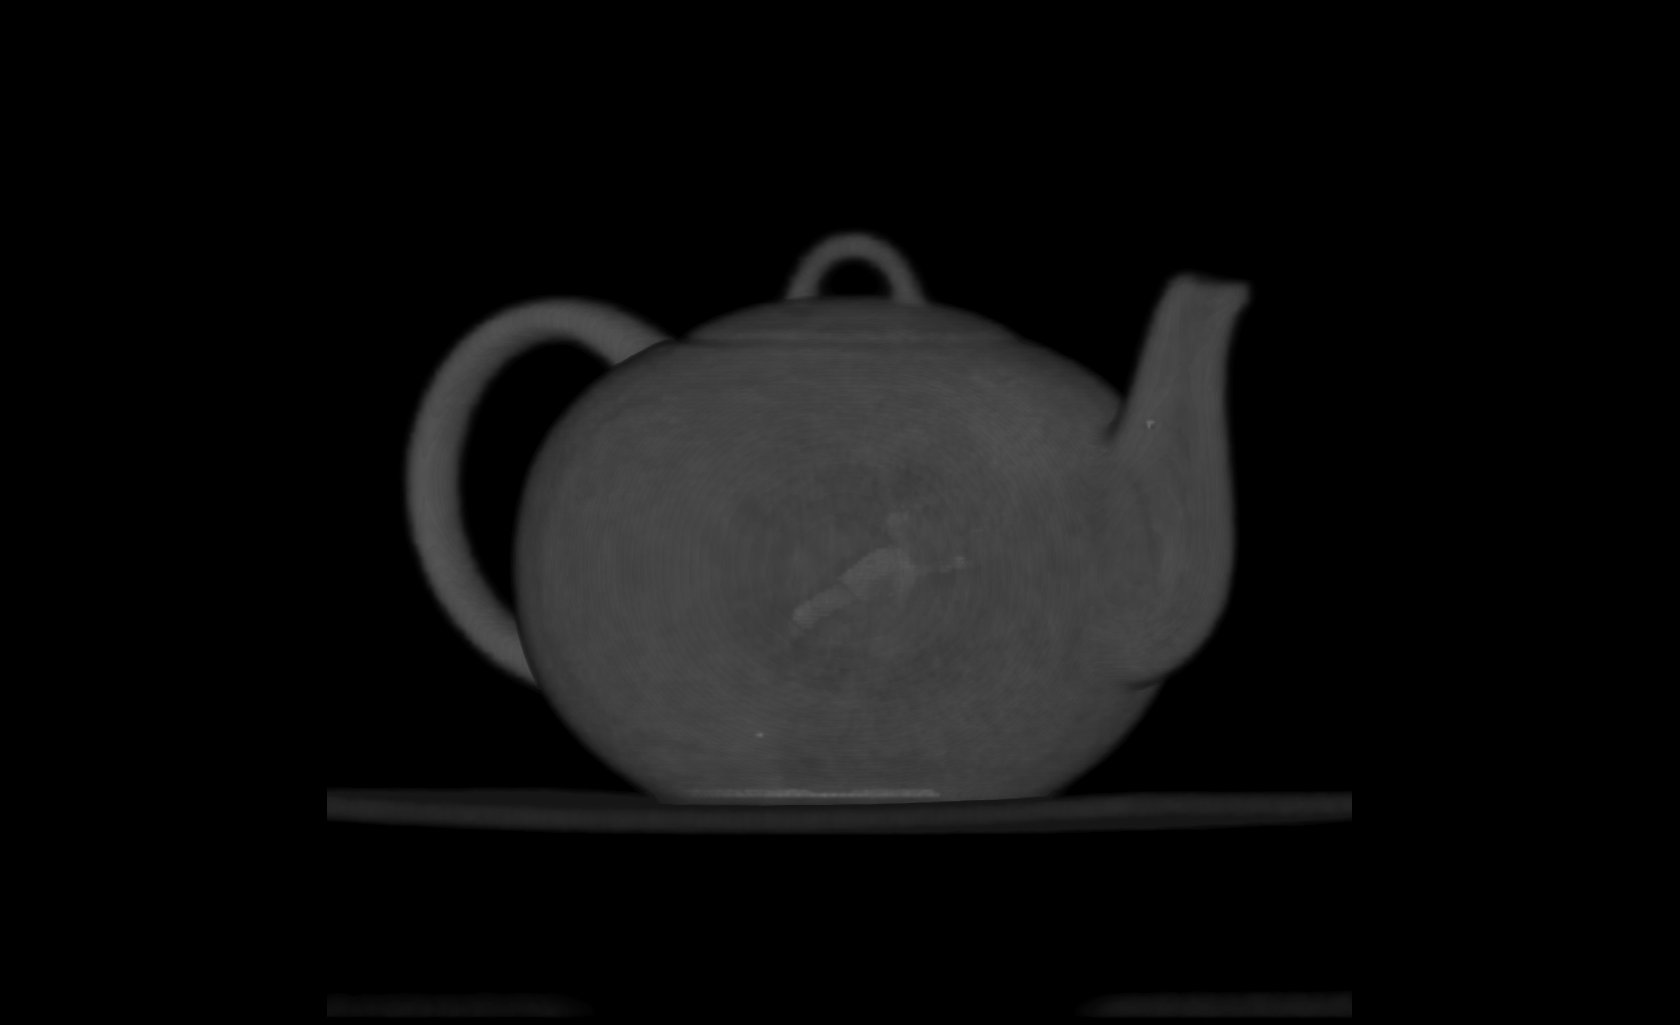
\includegraphics[width=0.325\linewidth]{./figures/experiments/denoisedVolumeImg.png}
    }\\
    \caption[Denoising 3D Grayscale Volume Data]{Denoising a 3D graysclae volume image
	\subref{fig:application_volume1_orig} Original image "BostonTeapot.raw", $256\times 256 \times 178$ px, 8 bit color depth
	\subref{fig:application_volume1_noise} Componentwise gaussian noise $\mu=0$, $\sigma=?$ added
	\subref{fig:application_volume1_denoised} Denoised, Proximal point with $\lambda=?$, $50$ PRPT steps
	\label{fig:application_volume1}
    }
\end{figure}
% subsection Volume images (end)

% section Color image denoising (end)

\FloatBarrier
\section{SO(2) and SO(3) images data} % (fold)
\label{sec:SO images data}

\subsection{Synthetic data} % (fold)
\label{sub:Synthetic data}
The following synthetic $SO(3)$ image is constructed in the following way. Let $\Omega=\lbrace 1,\ldots,30 \rbrace^2$ and define for every $(i,j)\in\Omega$
a rotation axis
\begin{equation}
	v = \begin{cases}
	    (2x,y,0)^{T}, & x>0.5\\
	    (0,2x,0.5)^{T}, & \text{ else}
	\end{cases},
\end{equation}
where $x=\frac{j}{30}, y=\frac{i}{30}$ and a rotation angle
\begin{equation}
    \alpha = \begin{cases}
	   x + y, & x > y\\
	   \frac{\pi}{2} + x - y, \text{ else}
    \end{cases}.
\end{equation}
Then assign the corresponding $SO(3)$ element representing a rotation by $\alpha$ and about $v$. Noise is added componentwise and the noisy matrix is
then projected back to $SO(3)$ using a the projector $P_{SO(n)}(A)=UV^{T}$ where $A=U\Sigma V^T$ is the singular value decomposition of $A$.

\begin{figure}[h!]
    \centering
    \subfloat[][Original]{
	\label{fig:application_so1_orig}
	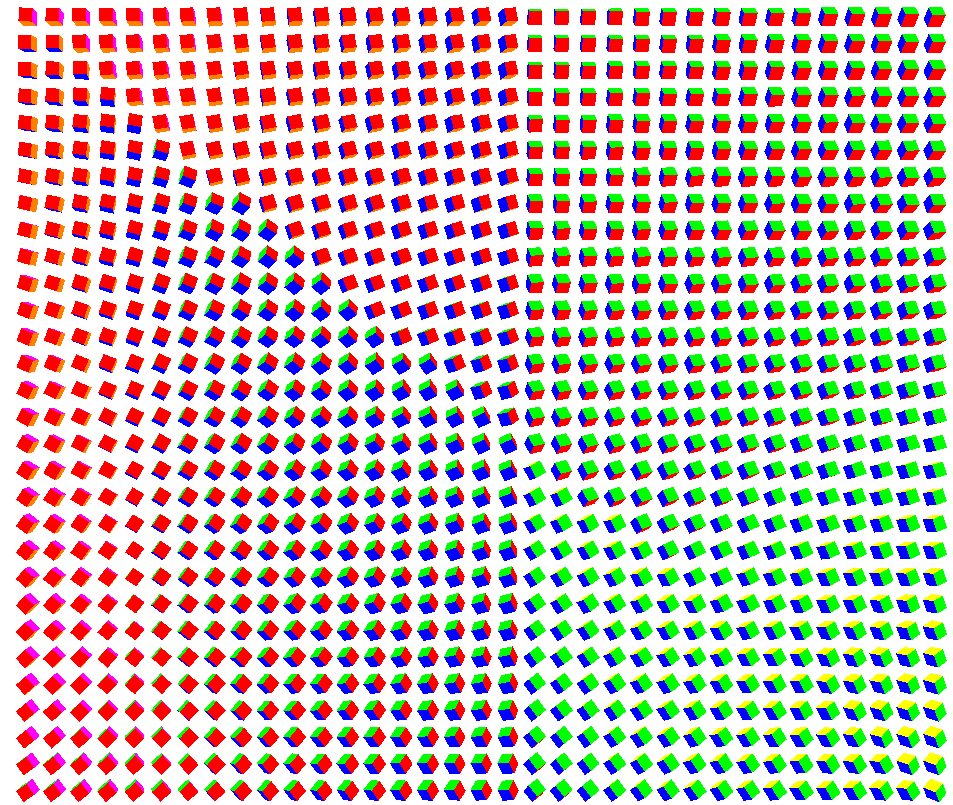
\includegraphics[width=0.325\linewidth]{./figures/experiments/son30x30original.png}
    }
    \subfloat[][Damaged]{
	\label{fig:application_so1_dam}
	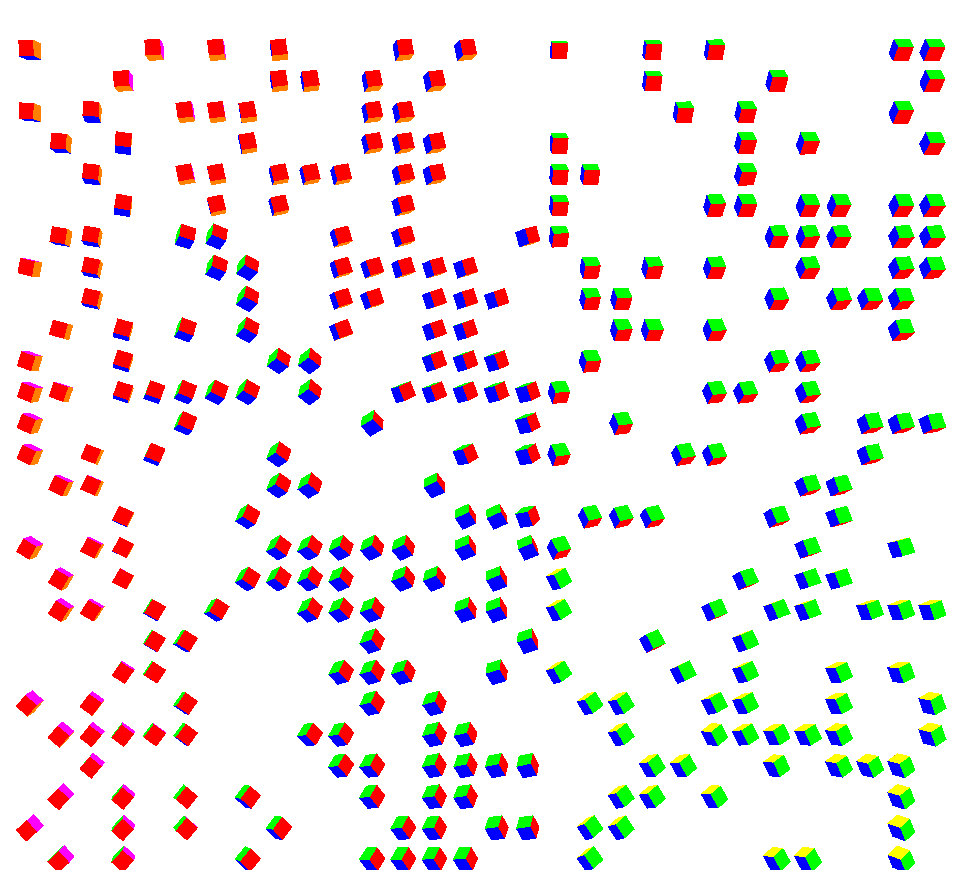
\includegraphics[width=0.325\linewidth]{./figures/experiments/son30x30damaged.png}
    }
    \subfloat[][Reconstructed]{
	\label{fig:application_so1_inp}
	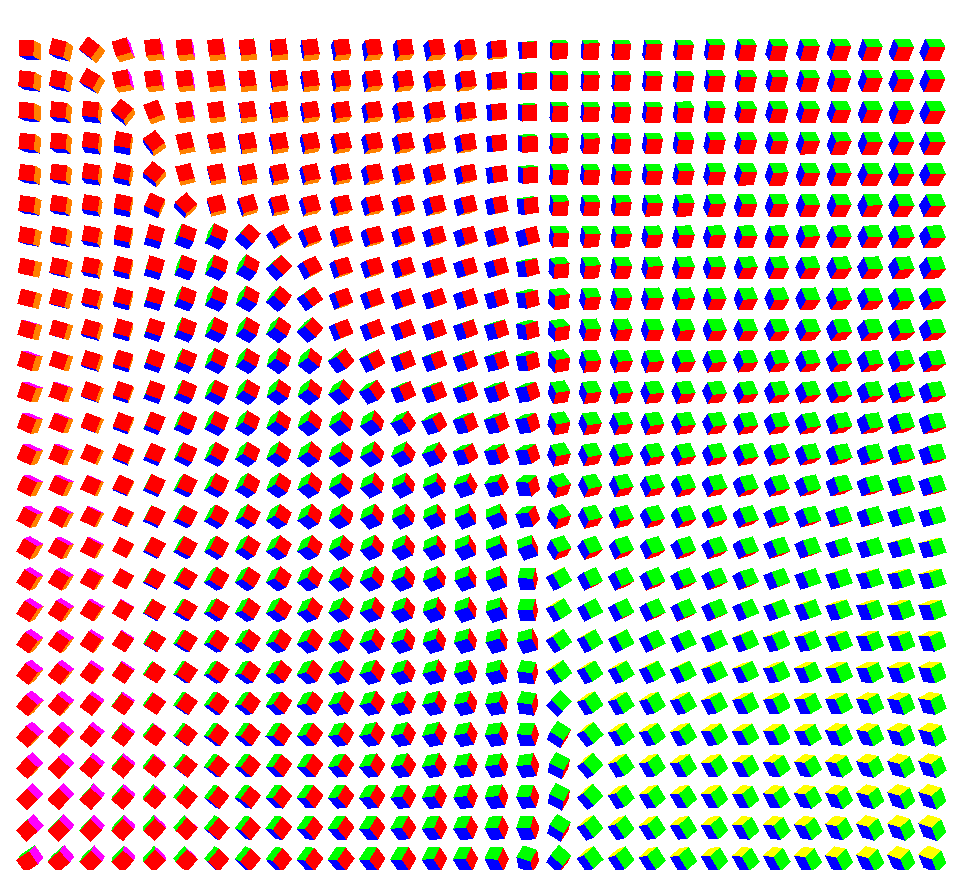
\includegraphics[width=0.325\linewidth]{./figures/experiments/son30x30inpainted.png}
    }\\
    \caption[Inpainting of synthetic SO(3) picture]{Inpainting of synthetic SO(3) picture
	\subref{fig:application_so1_orig} Original image: Synthetic, nonsmooth SO(3), $30\times 30$ px
	\subref{fig:application_so1_dam} Threshold $p=?$
	\subref{fig:application_so1_inp} Denoised, IRLS with $\lambda=?$, 5 IRLS steps, 1 Newton step per IRLS
	\label{fig:application_so1}
    }
\end{figure}

% subsection Synthetic data (end)

\FloatBarrier
\subsection{Fingerprint orientation data} % (fold)
\label{sub:Fingerprint orientation data}
Fingerprint matching is  based on extracting a set of particular features, called \emph{minutiae}, which uniquely define the fingerprint.
These features are usually ridge endpoint or ridge bifurkation points that are saved along with their position and orientation. This
means that prior to minutia detection and extraction the calculation of an orientation field is necessary.\\

For pictures of fingerprints this is just a special form of edge detection which can be done by calculating Sobel derivatives for every pixel.
Depending on the quality and noise level of the picture the computed orientation field can be very noisy itself which is another application
for our TV algorithms.\\

% subsection Fingerprint orientation data (end)
\begin{figure}[h!]
    \centering
    \subfloat[][Original]{
	\label{fig:application_fingerprint1_orig}
	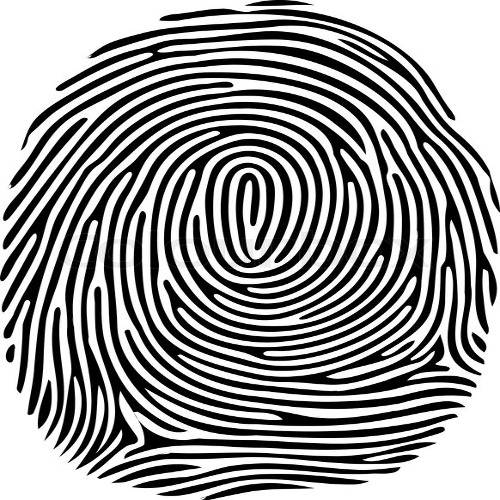
\includegraphics[width=0.325\linewidth]{./figures/experiments/fingerprint4.jpg}
    }
    \subfloat[][Computed Orientation field]{
	\label{fig:application_fingerprint1_noise}
	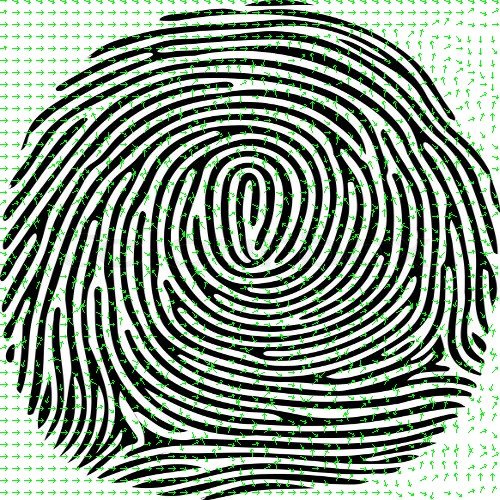
\includegraphics[width=0.325\linewidth]{./figures/experiments/input_fingerprint4.jpg}
    }
    \subfloat[][Denoised Orientation field]{
	\label{fig:application_fingerprint1_denoised}
	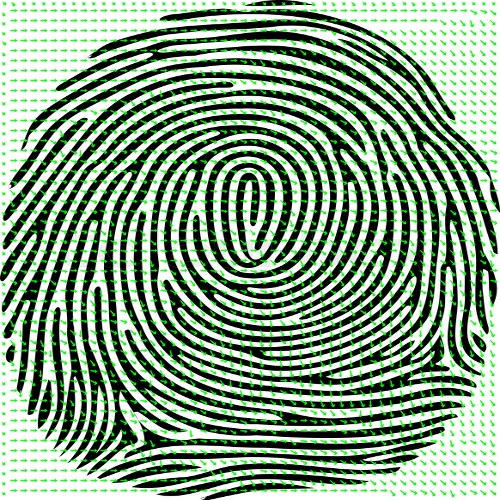
\includegraphics[width=0.325\linewidth]{./figures/experiments/denoised_fingerprint4.jpg}
    }\\
    \caption[Fingerprint orientation denoising]{Denoising a orientation field from a fingerprint, orientations represented by SO(2) elements
	\subref{fig:application_fingerprint1_orig} Original fingerprint 
	\subref{fig:application_fingerprint1_noise} Orientation field computed using Sobel derivatives PLACEHOLDER
	\subref{fig:application_fingerprint1_denoised} Denoised, IRLS with $\lambda=?$, $?$ IRLS steps, $?$ Newton steps per IRLS step PLACEHOLDER
	\label{fig:application_fingerprint1}
    }
\end{figure}

\FloatBarrier
\subsection{Reconstruction of a dense optical flow field} % (fold)
\label{sub:reconstructionDenseOpticalFlow}
An optical flow is the pattern of apparent motion between two consecutive frame of a video sequence. This may be the result of either an actual movement of the depicted object
or the result of a moving camera. Important applications are for example (anormal) motion detection, crowd behavior analysis, surveillance, video compression or image segmentation.\\
A \emph{dense} optical flow field can be interpreted as a vector field where each vector describes the displacement of a point between from one frame to the next. If
the set of points is retricted to only a few points of interest, a sparse feature set, we have \emph{sparse} optical flow.\\

In the following example, we only use a sparse feature set for tracking and flow computation in a short video sequence. The traffic scene was taken from a crowds/high density moving object data 
set provided by \cite{AliShah}. At first, we compute the sparse optical flow using the Lucas-Kanade algorithm \cite{LucasKanade} implemented in the OpenCV library. \\
For the set of tracked features 
$\mathcal{F}_1:=\lbrace{F^{(1)}_i\rbrace}_{i=1}^{400}\subset\Omega\subset\mathbb{R}^2$ in the first frame the algorithm tries to identify each feature in the second frame resulting in a set of
identified features $\mathcal{F}_2:=\lbrace{F^{(2)}_i\rbrace}_{i=1}^{N<400}\subset\Omega\subset\mathbb{R}^2$ and corresponding displacement vectors 
$\mathcal{V}_{12}:=\lbrace{V_i\,|\,V_i=F_i^{(2)}-F_i^{(1)}\rbrace}_{i=1}^{N}$.\\

We now assign to each pixel in our data an SO(2) element in the following way
\begin{align}
    \alpha_i &=\arctan\left(\frac{V^y_i}{V^x_i}\right) \\
    I(i,j) &= 
    \begin{cases}
    	\begin{pmatrix}
	    \cos\alpha_i    & -\sin\alpha_i\\
	    \sin\alpha_i    & \cos\alpha_i
	\end{pmatrix} & (i,j)\in \mathcal{F}_{2} \\
	0 & \text{ otherwise}
    \end{cases}
\end{align}

Since we want to reconstruct the dense flow, this is an inpainting problem and we have to perform scattered interpolation before running the algorithm. The result can be seen in 
Figure \ref{fig:application_flowfield1}.
\begin{figure}[h!]
    \centering
    \subfloat[][Original]{
	\label{fig:application_flowfield1_orig}
	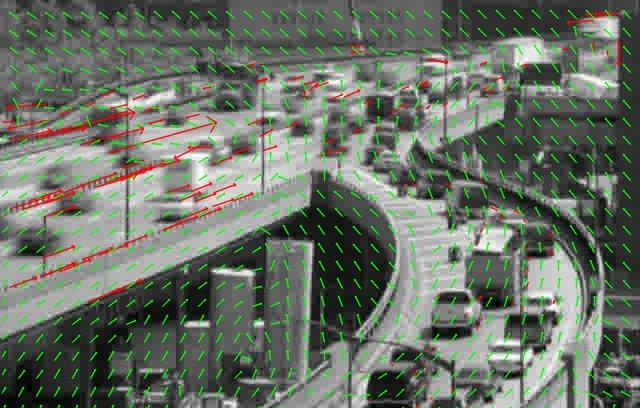
\includegraphics[width=0.325\linewidth]{./figures/experiments/reconstructed_optical_flow.jpg}
    }
    \subfloat[][Computed Sparse Flow field]{
	\label{fig:application_flowfield1_noise}
	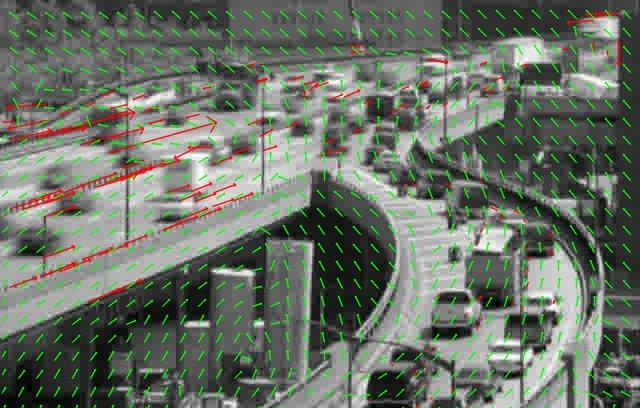
\includegraphics[width=0.325\linewidth]{./figures/experiments/reconstructed_optical_flow.jpg}
    }
    \subfloat[][Reconstructed orientation field]{
	\label{fig:application_flowfield1_denoised}
	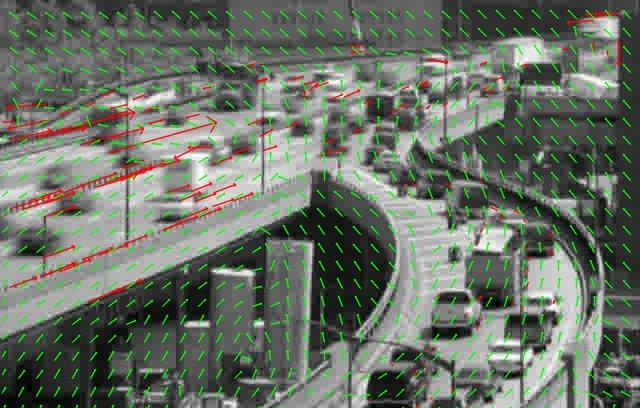
\includegraphics[width=0.325\linewidth]{./figures/experiments/reconstructed_optical_flow.jpg}
    }\\
    \caption[Dense optical flow reconstruction]{Reconstructing a dense flow from sparse feature tracking, orientations represented by SO(2) elements
	\subref{fig:application_flowfield1_orig} Frame of original video scene PLACEHOLDER
	\subref{fig:application_flowfield1_noise} Sparse features tracked using PLACEHOLDER
	\subref{fig:application_flowfield1_denoised} Reconstructed, IRLS with $\lambda=?$, $?$ IRLS steps, $?$ Newton steps per IRLS step
	\label{fig:application_flowfield1}
    }
\end{figure}

Of course the optimization could have also been performed on $S^1$. Furthermore, there is also a more direct, variational approach for the calculation of the flow field
which is also based on TV minimization but has a different fidelity term. This is one possibility for further extension of the library and is discussed in more detail in 
section \ref{sec:Extensions}

% subsection Calculation of a dense flow field (end)

% section SO(3) images data (end

\FloatBarrier
\section{SPD(3) image data} % (fold)
\label{sec:SPD(3) image data}

\subsection{Synthetic data} % (fold)
\label{sub:Synthetic data}
For the construction of the synthetic $SPD(3)$ image in Figure \ref{fig:application_spd1}, let $\Omega=\lbrace 1,\ldots,n \rbrace^2$ and define for every $(i,j)\in\Omega$
a rotation axis
\begin{equation}
	v = \begin{cases}
	    (x,y,2)^{T}, & x+y<1\\
	    (y,-x,1)^{T}, & \text{ else}
	\end{cases},
\end{equation}
where $x=\frac{j}{n}, y=\frac{i}{n}$ and a rotation angle
\begin{equation}
    \alpha = \begin{cases}
	   x+2y, & x+y<1\\
	   y+2x, \text{ else}
    \end{cases}.
\end{equation}
Let $R$ be the corresponding $SO(3)$ element representing a rotation by $\alpha$ and about $v$. Then define a diagonal matrix $D=\operatorname{diag}(x+0.2,y+0.2,0.5)$
and finally assign the matrix $A=R^{T}DR$ to the pixel.\\
Noise is then added by taking the matrix logarithm of every pixel, adding gaussian componentwise noise and apply the matrix exponential again.
\begin{figure}[h!]
    \centering
    \subfloat[][Original]{
	\label{fig:application_spd1_orig}
	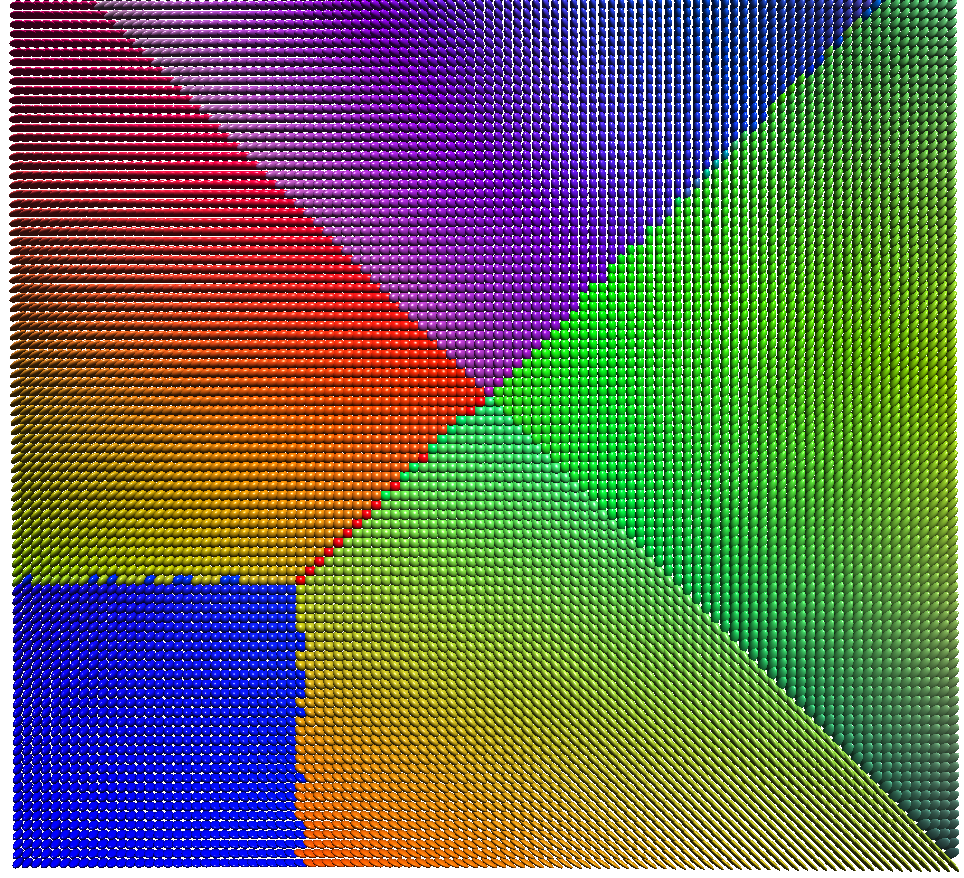
\includegraphics[width=0.325\linewidth]{./figures/experiments/spd_100x100.png}
    }
    \subfloat[][Damaged]{
	\label{fig:application_spd1_noise}
	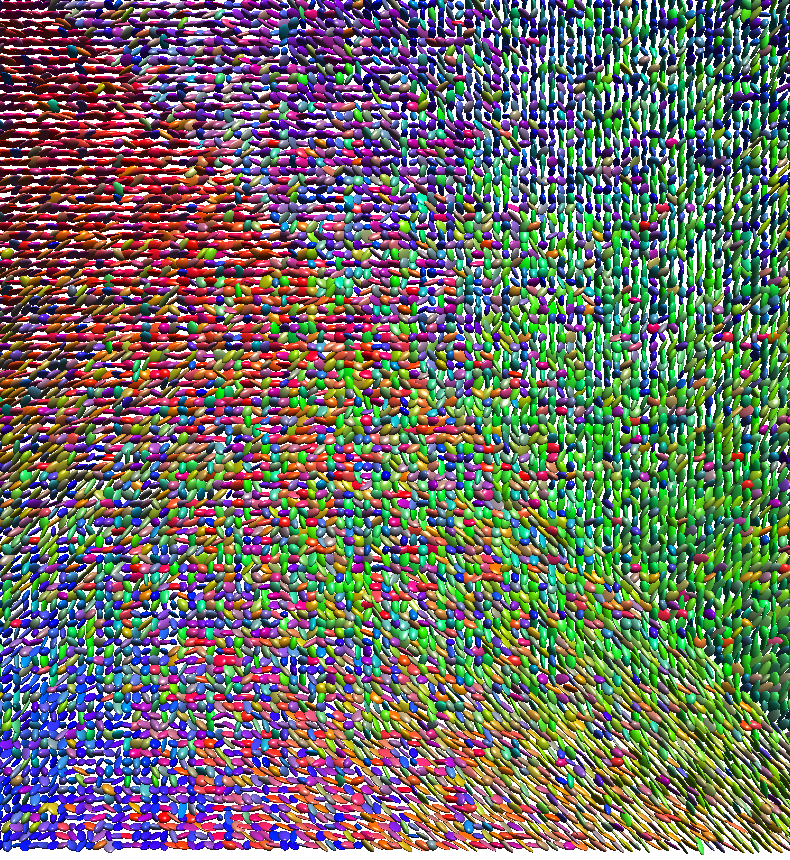
\includegraphics[width=0.325\linewidth]{./figures/experiments/noisy_spd100x100.png}
    }
    \subfloat[][Denoised]{
	\label{fig:application_spd1_denoised}
	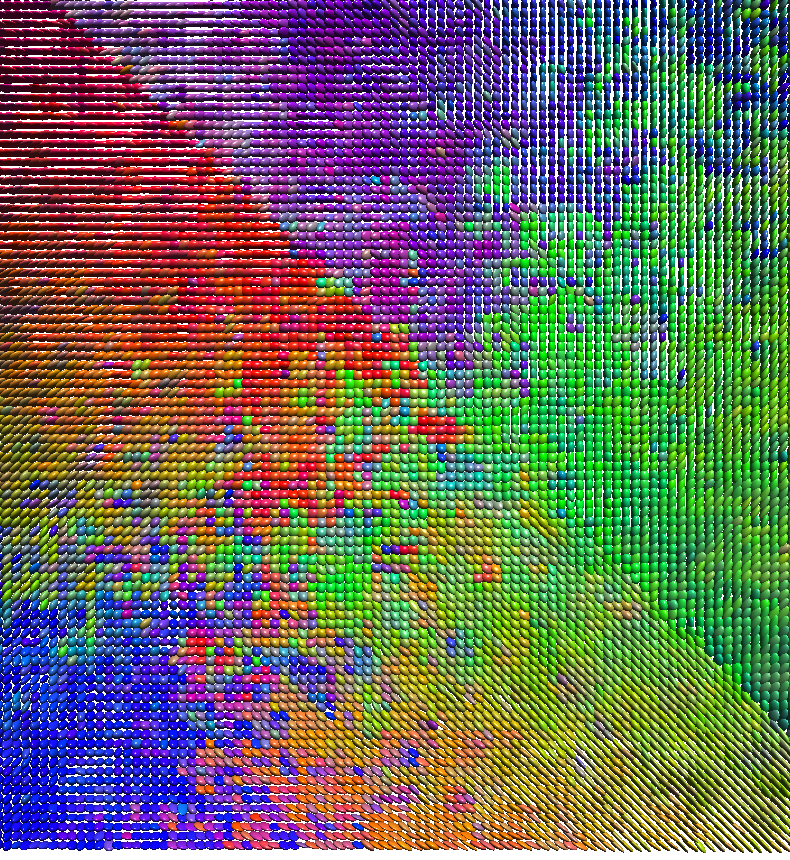
\includegraphics[width=0.325\linewidth]{./figures/experiments/denoised_spd100x100.png}
    }\\
    \caption[Denoising of synthetic SPD(3) picture]{Denoising of synthetic SPD(3) picture
	\subref{fig:application_spd1_orig} Original image: Synthetic, nonsmooth SPDO(3), $100\times 100$ px PLACEHOLDER
	\subref{fig:application_spd1_noise} Threshold $p=?$
	\subref{fig:application_spd1_denoised} Denoised, IRLS with $\lambda=?$, 5 IRLS steps, 1 Newton step per IRLS
	\label{fig:application_spd1}
    }
\end{figure}

% subsection Synthetic data (end)

\FloatBarrier
\subsection{Diffusion Tensor Magnetic Resonance Imaging} % (fold)
\label{sub:Diffusion Tensor MRI images}
Diffusion Tensor Magnetic Resonance Imaging (DT-MRI) is a medical imaging method which is able to non-invasively measure diffusion coefficients of water molecules
in living biological tissues. DT-MRI goes beyond CT or normal MR imaging methods which are only able to provide a single intensity value per voxel. Since water molecules
can move easier along, for example axons, connecting the neurons in the brain, than they can move across it, the resulting anisotropic diffusion pattern can provide a
lot of information about the structure of the brain.\\

DTI data sets are usually calculated from a set of diffusion weighted magnetic resonance imaging (DW-MRI) pictures.The basic magnetic resonance imaging works by applying an external magnetic along
the $z$-axis such that the proton spins in the tissue align either parallel or antiparallel to it, however, while still preceding around the $z$-axis with the so-called Lamor frequency.
An electromagnetic wave packet(HF-pulse) with that frequency leads to a collective state transition to a resonance state such that spin moments will be phase-synchronous before relaxing
back to their original orientation with respect to the external field. The magnetic field created by having synchronized moments can be measured by a coil where an electric potential will be created.
From the different relaxation times of different materials one can make conclusions about the structure of the tissue.\\

By applying an additional magnetic gradient field, the Lamor frequency of different layers of the probe can be modified such that only one layer of the material will resonate to the pulse.
This provides an additional positional resolution of the imaging process.\\

The DTI image is finally computed using the \emph{Stejskal-Tanner-equation} given by
\begin{equation}
    A(\mathbf{g})=A(0)\exp(-b\mathbf{g}^T\mathbf{D}\mathbf{g})
\end{equation}
where $A(\mathbf{g})$ denotes the signal strength, $\mathbf{g}$ the magnetic gradient field and $b$ some measurement related parameters. Solving this equation for $\mathbf{D}$ finally
leads to desired $SPD(3)$ matrix describing the diffusion coefficents and directions.\\
% subsection Diffusion Tensor MRI images (end)
\begin{figure}[h!]
    \centering
    \subfloat[][Noisy]{
	\label{fig:application_dti1_noise}
	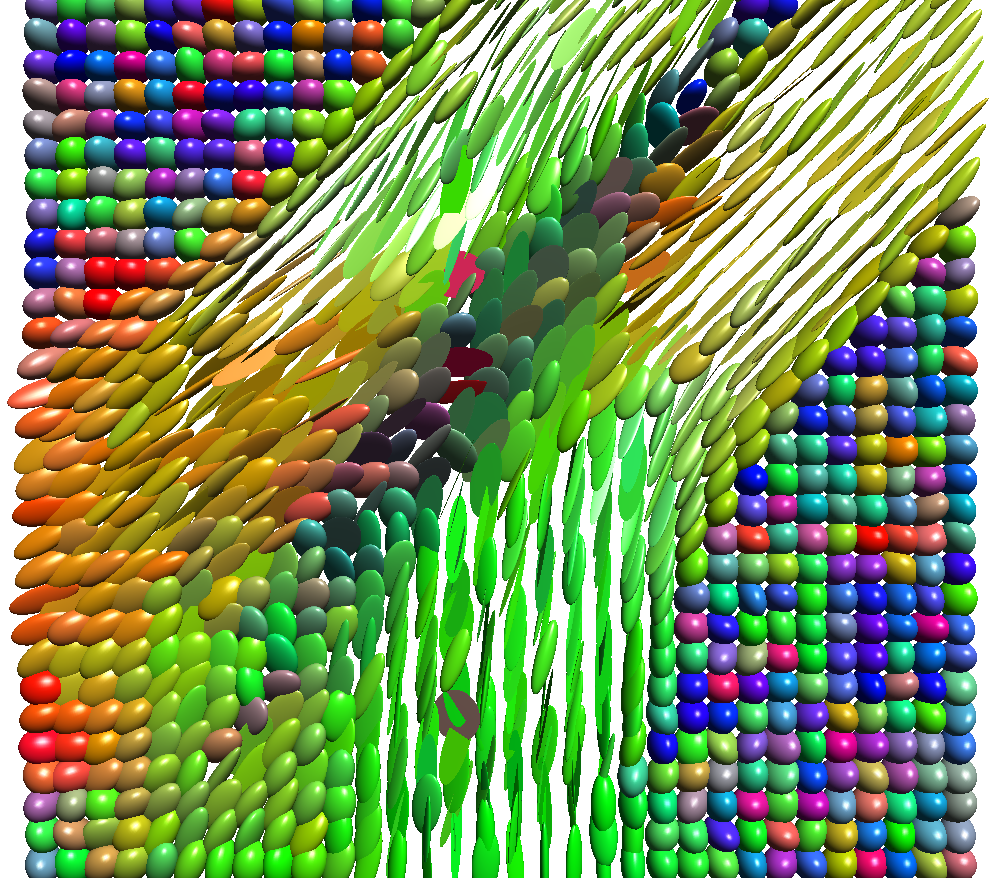
\includegraphics[width=0.5\linewidth]{./figures/experiments/noisy_dti32x32.png}
    }
    \subfloat[][Denoised]{
	\label{fig:application_dti1_denoised}
	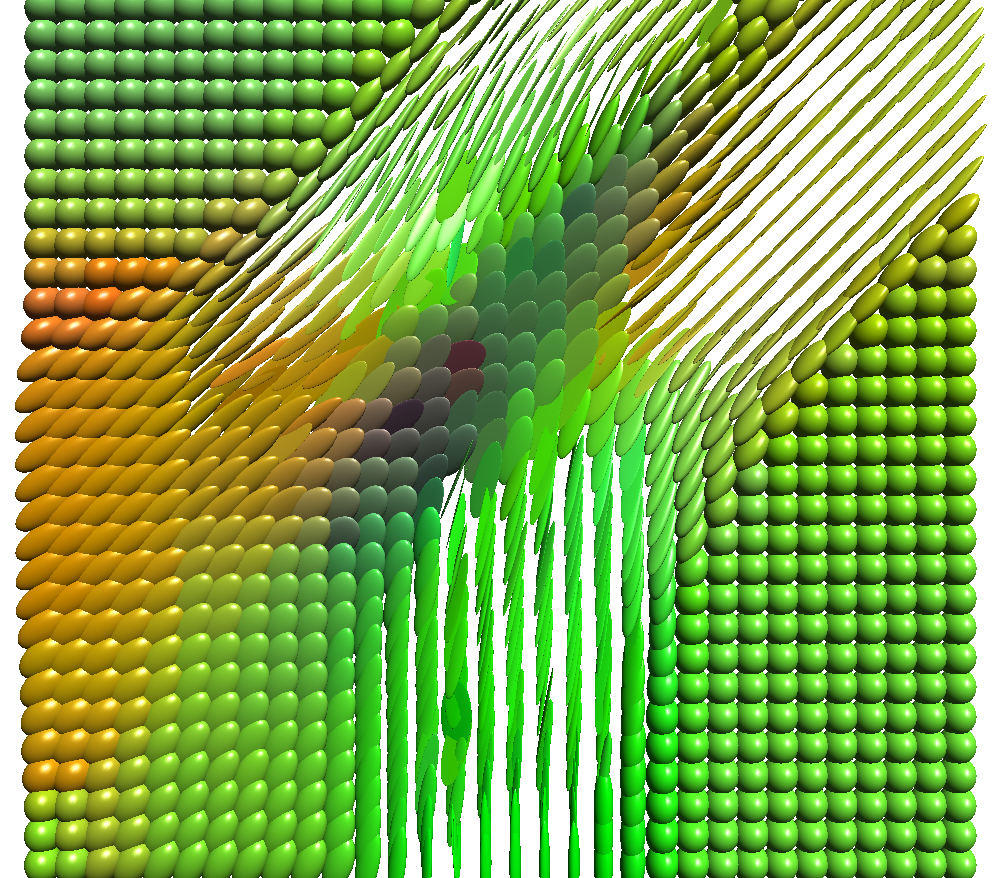
\includegraphics[width=0.5\linewidth]{./figures/experiments/denoised_dti32x32.png}
    }\\
    \caption[Denoising DT-MRI data]{Denoising a DT-MRI image with pixel in SPD(3)
	\subref{fig:application_dti1_noise} Original DTI data, 32x32 pixel
	\subref{fig:application_dti1_denoised} Denoised, IRLS with $\lambda=?$, $?$ IRLS steps, $?$ newton steps per IRLS step
	\label{fig:application_dti1}
    }
\end{figure}

In Figure \ref{fig:application_dti1} the IRLS minimizer is applied to DTI data set provided by Barmpoutis \cite{barmpoutis}.
On clearly identify regions of high anistropy in the picture, where the molecules are forced to diffuse in one preferred direction.
The areas dominated mainly by green spheres correspond to approximately isotropic diffusion which means that there are no obstacles like axons in the brain in the 
immediate proximity of the water molecules.\\


\FloatBarrier
\subsection{3D DT MRI data} % (fold)
\label{sub:3DDTMRIdata}
% subsection 3D DT MRI data (end)

Finally, in Figure \ref{fig:application_dti2_noise} we show a 3D DTI image. Shown is a $16\times 16\times 16$ cube from a human brain scan and we used the proximal point algorithm for denoising. 
The brain dataset is a courtesy of Gordon Kindlmann at the Scientific Computing and Imaging Institute, University of Utah, 
and Andrew Alexander, W. M. Keck Laboratory for Functional Brain Imaging and Behavior, University of Wisconsin-Madison. 
\begin{figure}[h!]
    \centering
    \subfloat[][Original]{
	\label{fig:application_dti2_noise}
	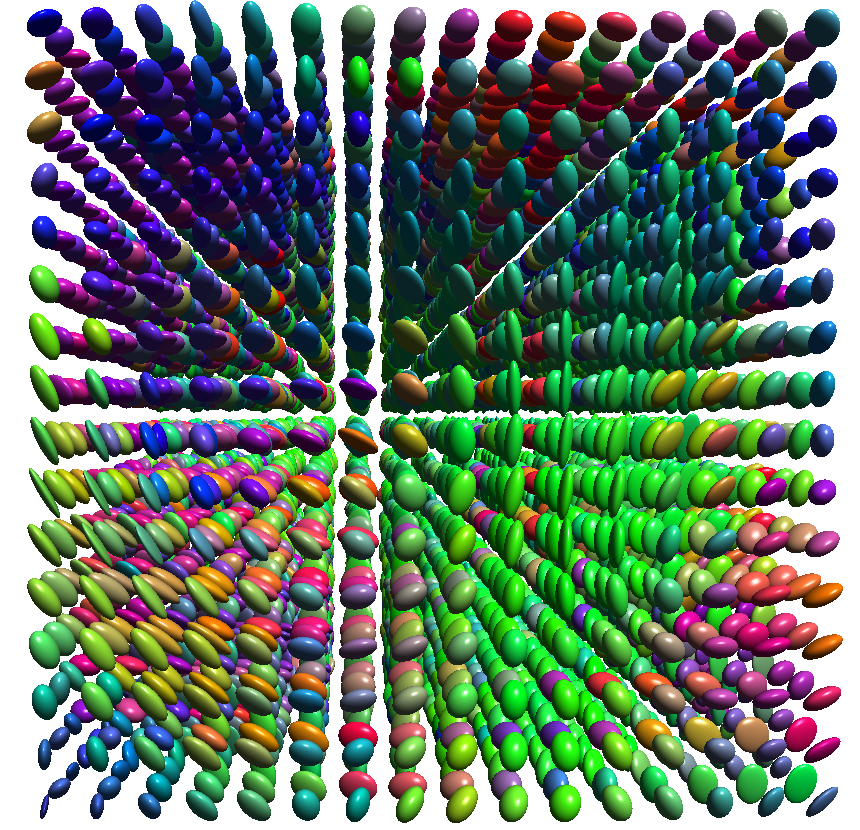
\includegraphics[width=0.5\linewidth]{./figures/experiments/noisy_dti3d16x16x16.png}
    }
    \subfloat[][Denoised]{
	\label{fig:application_dti2_denoised}
	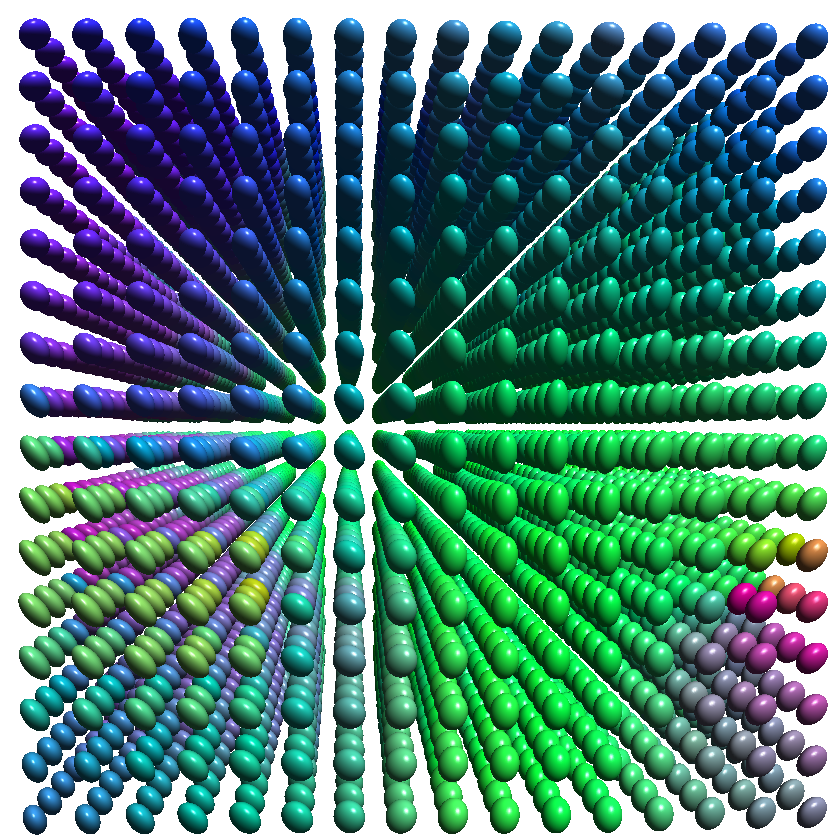
\includegraphics[width=0.5\linewidth]{./figures/experiments/denoised_dti3d16x16x16.png}
    }\\
    \caption[Denoising 3D DTI-MRI data]{Denoising a 3D DT-MRI image with pixel in SPD(3)
	\subref{fig:application_dti2_noise} Original, $16\times 16\times 16$ pixel 
	\subref{fig:application_dti2_denoised} Denoised, Proximal point with $\lambda=0.7$, 50 PRPT steps
	\label{fig:application_dti2}
    }
\end{figure}

% section SPD(3) image data (end)
\FloatBarrier
\section{Performance profiling of the library} % (fold)
\label{sec:Performance profiling of the library}
In this section we analyze the performance hotspots of the library for the case of the IRLS minimizer. This is done using the Linux tool \emph{perf} which monitors a variety of different
performance metrics during the execution of a program, like CPU cycles, cache or branch misses. To identify the hotspots, where most of the computation is spent, the number of CPU cycles is
usually the most suitable metric.\\

Concerning the computational complexity of operations performed on single pixels the Euclidian manifold is certainly the least demanding, because exponential and logarithm map are just 
addition and subtraction and the second derivative of the distance function is just two times the identity matrix. At the other end of the spectrum is the $SPD$ manifold where
computations usually involve multiple matrix multiplications, exponential, logarithms and derivatives thereof. For the analysis we thus choose these two representatives and compared
different image sizes.\\

For the Euclidian manifold we choose the "Lena" and "Mathematicians" pictures already considered in the example above. Minimization in the first case took approximately 9 seconds and 270 seconds in
the second case. The data is shown in Table \ref{table:perf_euc} where the first column denotes the percentage of CPU cycles spent in the routine specified in the second column 
while the last column denotes the (external) library to which it belongs. Only the top six routines are shown since the individual share of the others was in most cases less than 1 \%. \\

We can observe that in both cases computation is dominated by the Basic Linear Algebra Subprograms (BLAS) Library. Those in turn are called by the CHOLMOD library which solves the sparse
linear system using Cholesky factorization. The only contribution that does not belong to the linear system is the multithreading overhead from the OpenMP (OMP) library in the smaller picture.
We see, however, that for the increased system size the overhead becomes negligibly small such that for both problem sizes more than two thirds of the total computation time is for solving the linear
system. For the larger picture this share even grows to more than 75\% and could be expected to do so for yet larger images.\\

\begin{table}[h!]
\centering
\footnotesize
\setlength{\tabcolsep}{3pt}
\subfloat[][$361\times 361$]{
	\label{table:perf_lena}
	\begin{tabular}{rll}
	\hline
	Share & Routine & Library \\
	\hline
	25.73& DGEMM(matrix matrix multiply)& BLAS\\
	20.71& DSYRK(symmetric rank-k update)& BLAS\\
	13.86& Multihreading overhead& OMP\\
	11.57& DTRSM(solve triangular system)& BLAS\\
	3.23& DGEMV(matrix vector multiply)& BLAS\\
	3.22& cholmod\textunderscore super\textunderscore numeric & CHOLMOD\\
	\hline
	\end{tabular}
}\,
\subfloat[][$1280\times 1024$]{
	\label{table:perf_mathematicians}
	\begin{tabular}{rll}
	\hline
	Share & Routine & Library\\
	\hline
	30.37& DGEMM(matrix matrix multiply)& BLAS\\
	27.70& DSYRK(symmetric rank-k update)& BLAS\\
	14.65& DTRSM(solve triangular sytem)& BLAS\\
	2.79& set\_rom\_triplets(sparse initialization)& Eigen\\
	2.18& CreateCoarserGraph & METIS\\
	1.68& cholmod\_super\_numeric & CHOLMOD\\
	\hline
	\end{tabular}
}
\caption[]{Share of total CPU cycles for IRLS minimization over $M=\mathbb{R}^3$
\subref{table:perf_lena}"Lena.jpg", $361\times 361$ pixel
\subref{table:perf_mathematicians}"Mathematicians.jpg", $1280\times 1024$ pixel
\label{table:perf_euc}
}
\end{table}

For the $SPD(n)$ manifold the situation, shown in Table \ref{table:perf_spd} and Table \ref{table:perf_spd300}, looks a bit different at first. 
For the smallest problem size of $30\times 30$ pixels, there are dominating parts. The largest contribution is the from multithreading which is to be expected
for such a small picture and which consequently vanishes for larger images. 
The next important routine is our implementation of the matrix logarithm Fr\'{e}chet derivative while the remaining Eigen routines in the
list are auxiliary functions for solving triangular matrix functions which are need for the computation of matrix square roots, logarithms and of course also the
Fr\'{e}chet derivatives. With increasing problem size, we can again observe how the BLAS routines move to the top of the list, even though their share only amounts 
to a fifth of all CPU cycles for the $300\times 300$ pixel image. \\

\begin{table}[h!]
\centering
\footnotesize
\setlength{\tabcolsep}{3pt}
\subfloat[][$30\times 30$]{
	\label{table:perf_spd30}
	\begin{tabular}{rll}
	\hline
	Share & Routine & Library \\
	\hline
	11.6& Multithreading overhead& OMP\\
	7.73& MatrixLogarithmFrechetDerivative& TVMTL\\
	6.77& reduceToTriangularForm& Eigen\\
	6.55& gebp\_kernel(matrix blocking)& Eigen\\
	6.18& triangular\_solve\_matrix& Eigen\\
	4.55& triangular\_solve\_matrix& Eigen\\
	\hline
	\end{tabular}
}\,
\subfloat[][$100\times 100$]{
	\label{table:perf_spd100}
	\begin{tabular}{rll}
	\hline
	Share & Routine & Library\\
	\hline
	11.60& MatrixLogarithmFrechetDerivative& TVMTL\\
	7.72& reduceToTriangularForm& Eigen\\
	6.77& gebp\_ kernel(matrix blocking)& Eigen\\
	6.55& triangular\_solve\_matrix& Eigen\\
	6.18& triangular\_solve\_matrix& Eigen\\
	4.55& DGEMM(matrix matrix multiply)& BLAS\\
	\hline
	\end{tabular}
}
\caption[]{Share of total CPU cycles for IRLS minimization over $M=SPD(3)$
\subref{table:perf_spd30} Synthetic $SPD(3)$ , $30\times 30$
\subref{table:perf_spd100} Synthetic $SPD(3)$ , $100\times 100$
\label{table:perf_spd}
}
\end{table}


\begin{table}[h!]
\centering
\footnotesize
\begin{tabular}{rll}
\hline
Share & Routine & Library\\
\hline
11.31& DGEMM(matrix matrix multiply)& BLAS\\
9.73& MatrixLogarithmFrechetDerivative& TVMTL\\
9.19& DSYRK(symmetric rank-k update)& BLAS\\
6.60& reduceToTriangularForm& Eigen\\
5.73& gebp\_kernel(matrix blocking)& Eigen\\
5.55& triangular\_solve\_matrix& Eigen\\
\hline
\end{tabular}
\caption{Share of total CPU cycles for IRLS minimization of synthetic $SPD(3)$ , $300\times 300$ pixel, $M=SPD(3)$
\label{table:perf_spd300}
}
\end{table}

We can conclude that solving the linear system is the most performance relevant aspect of the IRLS minimizer. The share is even higher for $SO(n)$ and $S^n$, where the SuperLU library is used, 
since the corresponding sparse Hessian is not symmetric resulting in a further increased operations count. If a good preconditioner is found, iterative solvers might speed up the computation, 
the standard diagonal and incomplete LU preconditioner provided by the Eigen library, however, performed worse than the direct solvers from the SparseSuite library collection. Finally, for
the matrix-valued manifolds, the implementation of the Fr\'{e}chet derivative could potentially be improved.


% section Performance profiling of the library (end)


\FloatBarrier
\section{Comparison IRLS and Proximal Point minimizers} % (fold)
\label{sec:Comparison IRLS and Proximal Point minimizers}

To make a comparison with the tests performed in \cite{SprecherIRLS} using the original Matlab implementation to a certain degree possible, we choose 
almost the same set of test images (Figure \ref{fig:comparison_testimages}) but additionally also some larger versions of the pictures for the more interesting 
case of the matrix manifolds $SO(3)$ and $SPD(3)$. Both, the IRLS and the proximal point minimizers are implemented using the same manifold classes and utilize the
same pixel-wise parellelization techniques such that there is no obvious bias in this comparison.\\

The synthetic images are created using the formulas already described in the examples above. To each picture we add component-wise gaussian noise with zero mean and
standard deviation of $\sigma=0.2$. With that noise level no smoothing is needed for the IRLS algorithm to converge. 
For each picture we compute the value of the functional after each iteration and the error relative to an approximate minimizer $u^*$
which is computed using the IRLS algorithm with $\lambda=0.2$, 20 IRLS steps and one newton step per reweighting. This error is defined as
\begin{equation}
e^{(k)}=\sum_{i,j}\;d^2(u^{(k)}_{ij},u^*_{ij})
\end{equation}
where $d^2(\cdot,\cdot)$ denotes the squared Riemannian distance function of the appropriate manifold. For the iterations itself we use 15 iterations for IRLS and 500 for proximal point with
the sequence $\mu_k=3k^{-0.95}$ (see \cite{Weinmann} for details on this sequence) for all experiments. \\

\begin{figure}[h!]
    \centering
    \subfloat[][$\mathbb{R}^3$]{
	\label{fig:comparison_eucimg}
	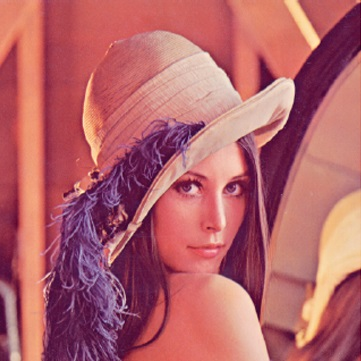
\includegraphics[width=0.2\linewidth]{./figures/experiments/Lena.jpg}
    }
    \subfloat[][$S^2$]{
	\label{fig:comparison_s2img}
	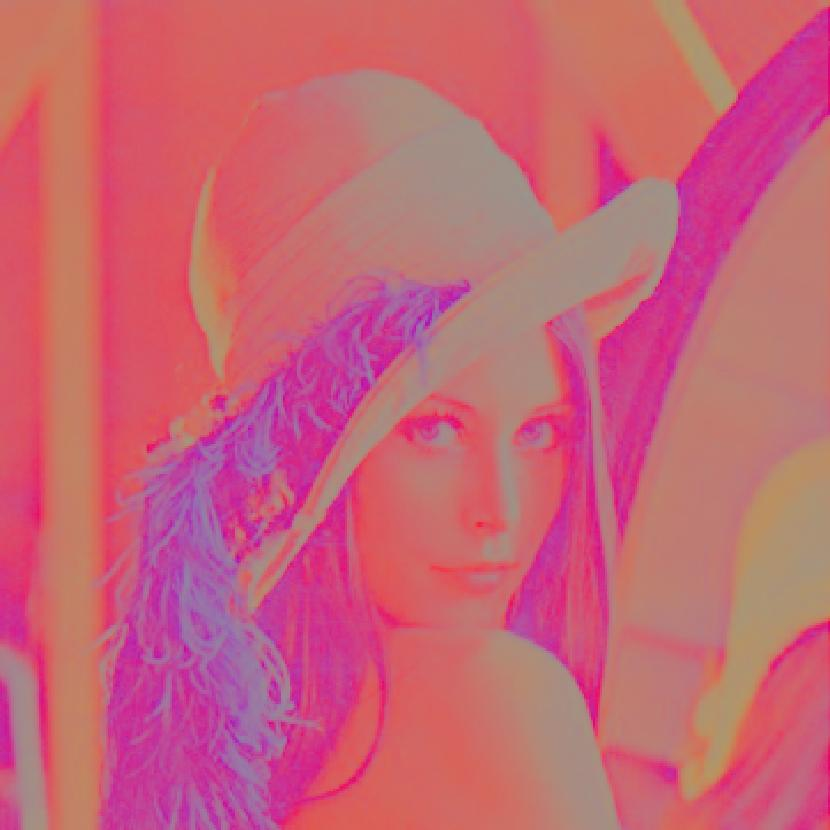
\includegraphics[width=0.2\linewidth]{./figures/experiments/chroma_Lena.jpg}
    }
    \subfloat[][$SO(3)$]{
	\label{fig:comparison_sonimg}
	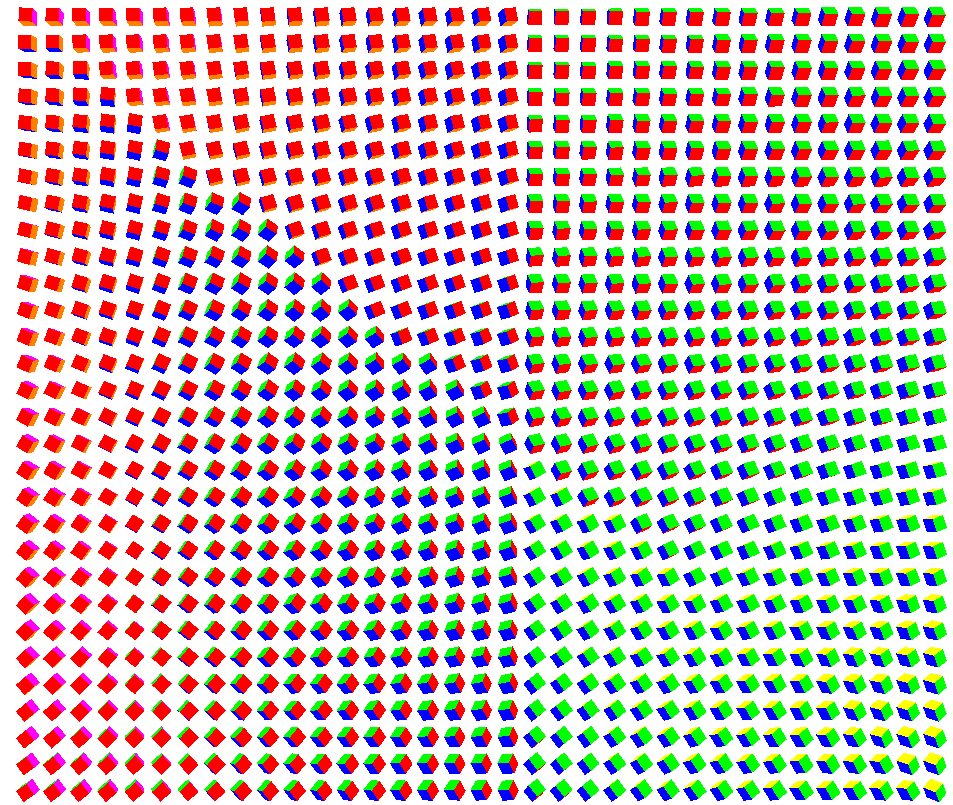
\includegraphics[width=0.3\linewidth]{./figures/experiments/son30x30original.png}
    }
    \subfloat[][$SPD(3)$]{
	\label{fig:comparison_spdimg}
	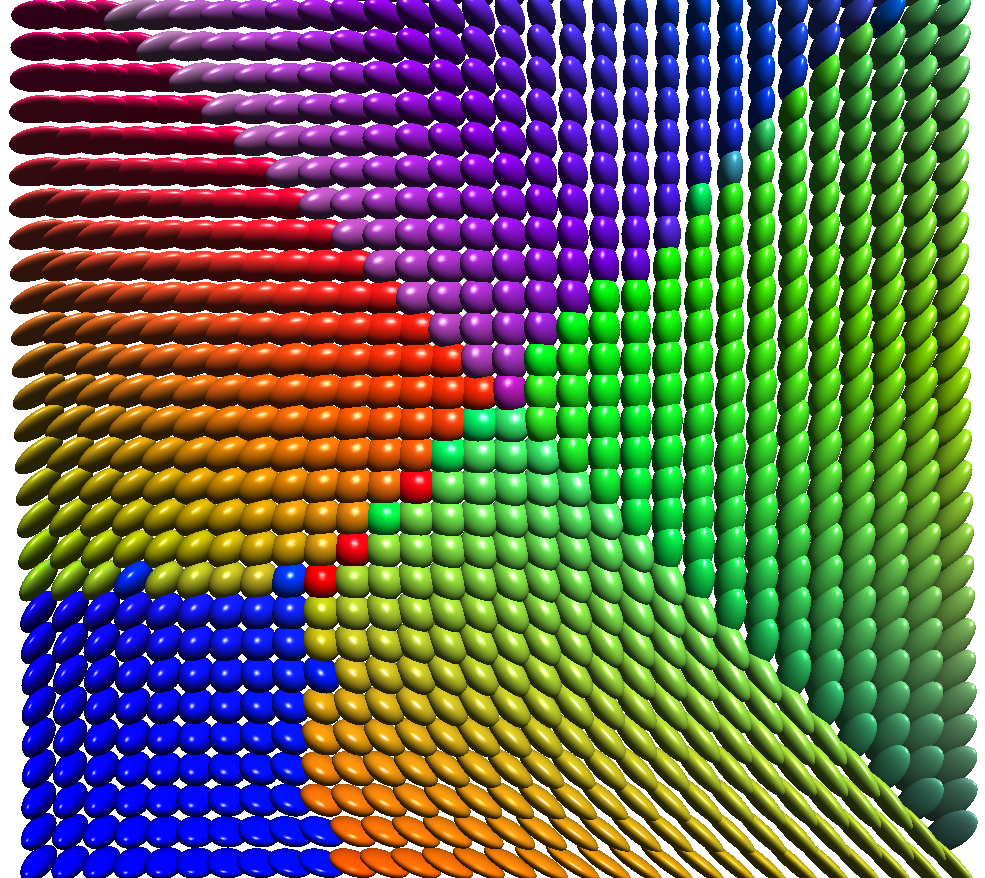
\includegraphics[width=0.3\linewidth]{./figures/experiments/spd_30x30.png}
    }\\
    \caption[Test images]{ Test images for the IRLS \& PRPT comparison
	\subref{fig:comparison_eucimg}  "Lena.jpg", $361\times 361$ px, $\mathbb{R}^3$-valued
	\subref{fig:comparison_s2img} Chromaticity part of "Lena.jpg", $S^2$-valued
	\subref{fig:comparison_sonimg} Synthetic $30\times30$ and $100\times100$ image, $SO(3)$-valued
	\subref{fig:comparison_spdimg} Synthetic $30\times30$ and $100\times100$ image, $SPD(3)$-valued
	\label{fig:comparison_testimages}
    }
\end{figure}


\begin{figure}[h!]
    \centering
    \subfloat[][Euclidian $\mathbb{R}^3$ - Functional]{
	\label{fig:comparison_eucJ}
	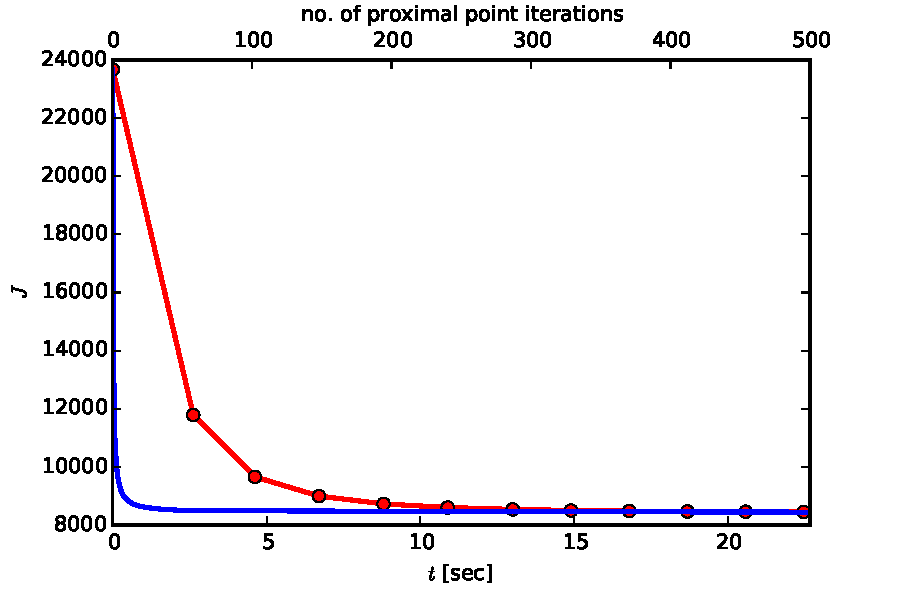
\includegraphics[width=0.5\linewidth]{./figures/experiments/Lena_361x361_J.pdf}
    }
    \subfloat[][Euclidian $\mathbb{R}^3$ - Error]{
	\label{fig:comparison_eucE}
	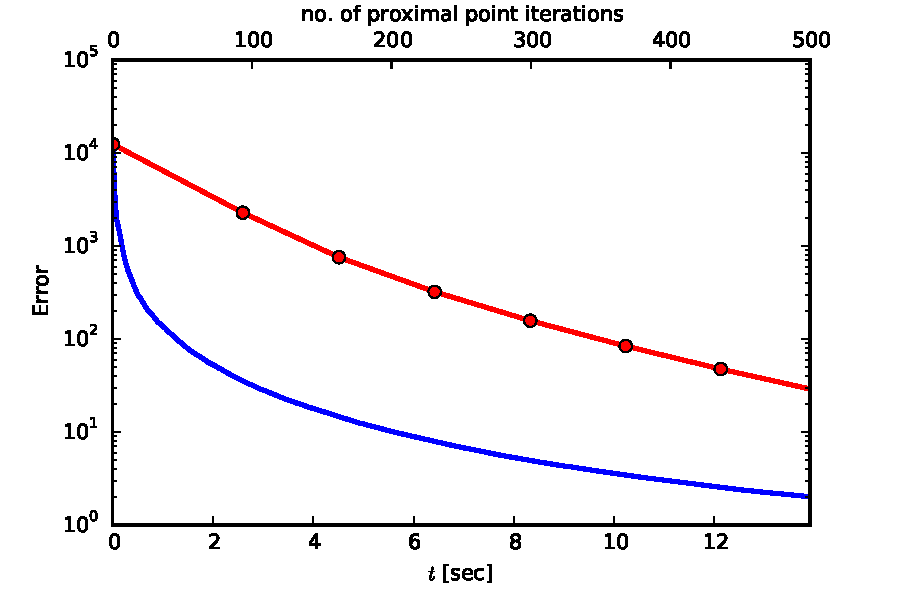
\includegraphics[width=0.5\linewidth]{./figures/experiments/Lena_361x361_Err.pdf}
    }\\
    \subfloat[][Sphere $S^2$ - Functional]{
	\label{fig:comparison_s2J}
	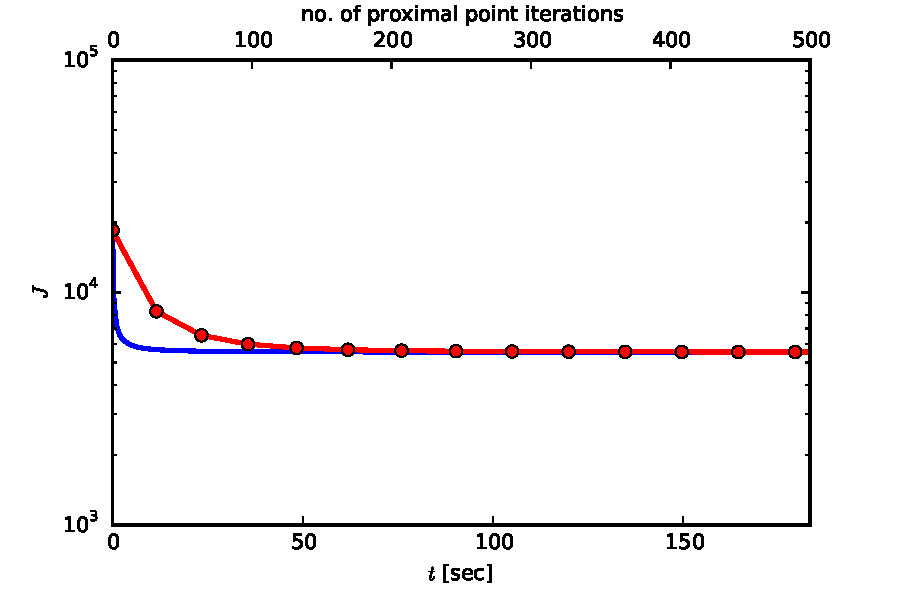
\includegraphics[width=0.5\linewidth]{./figures/experiments/Lena_361x361CBR_J.pdf}
    }
    \subfloat[][Sphere $S^2$ - Error]{
	\label{fig:comparison_s2E}
	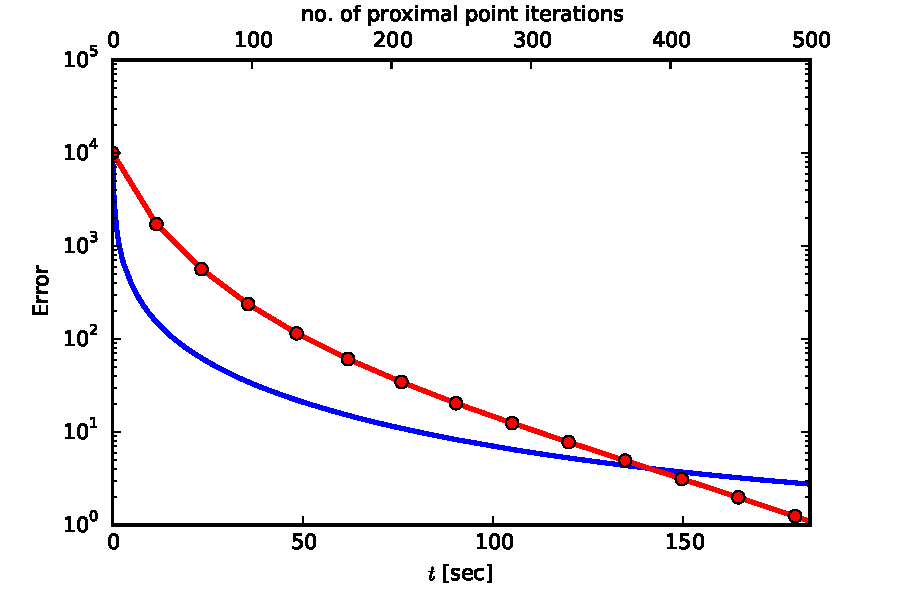
\includegraphics[width=0.5\linewidth]{./figures/experiments/Lena_361x361CBR_Err.pdf}
    }\\
    \caption[Comparison IRLS \& PRPT for Euclidian $\mathbb{R}^3$ and $S^2$]{Comparison of functional value and errors for IRLS and PRPT minimizers.
	The red circles correspond to IRLS iterations while the line without any markers belongs to the proximal point iterations.
	\subref{fig:comparison_eucJ} Functional values for "Lena" minimized over $\mathbb{R}^3$
	\subref{fig:comparison_eucE} Errors relative to minimizer for "Lena"
	\subref{fig:comparison_s2J} Functional values for color part of "Lena" minimized over $\mathbb{S}^2$
	\subref{fig:comparison_s2E} Errors relative to minimizer for color part "Lena"
	\label{fig:comparison_euc_s2}
    }
\end{figure}

Figure \ref{fig:comparison_euc_s2} shows the results for Euclidian space $\mathbb{R}^3$ and the sphere $S^2$. IRLS needs only five iterations where proximal point needs more than 200
but nevertheless proximal wins in terms of speed. This result can be interpreted with respect the performance analysis conducted in the previous section. Most manifold quantities can
be computed using only addition and subtraction and which includes the geodesic interpolation that proximal point has to perform in every direction as well as the computation for derivatives
for IRLS. The effort of doing these two task seems intuitively similar. At the end for that process, however, proximal point only has to compute simple arithmetic means while IRLS has to 
solve the sparse system which was shown to be the dominant part of the computation and thus probably more time consuming than the averaging procedure. For $S^2$, in comparison, one
can already see IRLS catching up.\\

\begin{figure}[h!]
    \centering
    \subfloat[][$SO(3)$ (30$\times$30) - Functional]{
	\label{fig:comparison_son30J}
	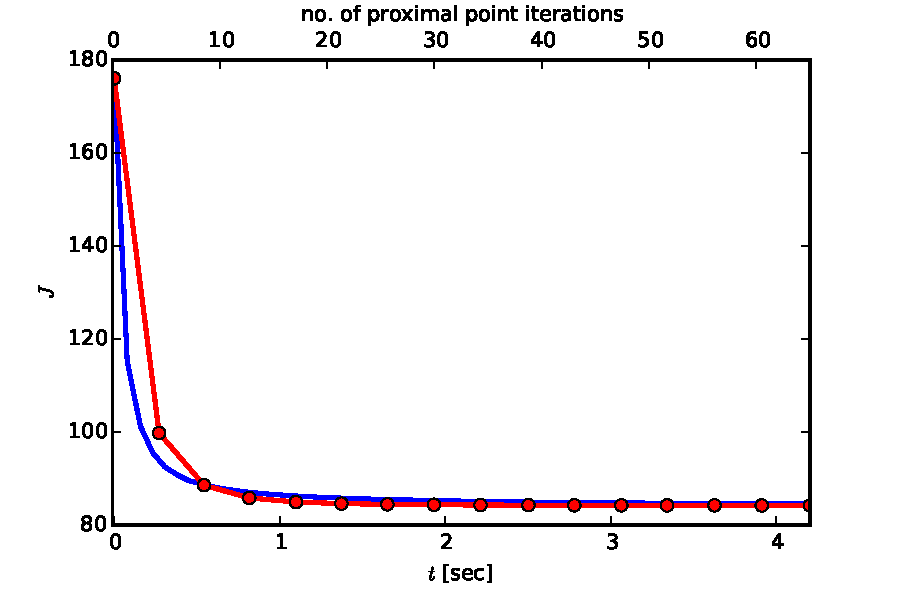
\includegraphics[width=0.5\linewidth]{./figures/experiments/SON_30x30_J.pdf}
    }
    \subfloat[][$SO(3)$ (30$\times$30) - Error]{
	\label{fig:comparison_son30E}
	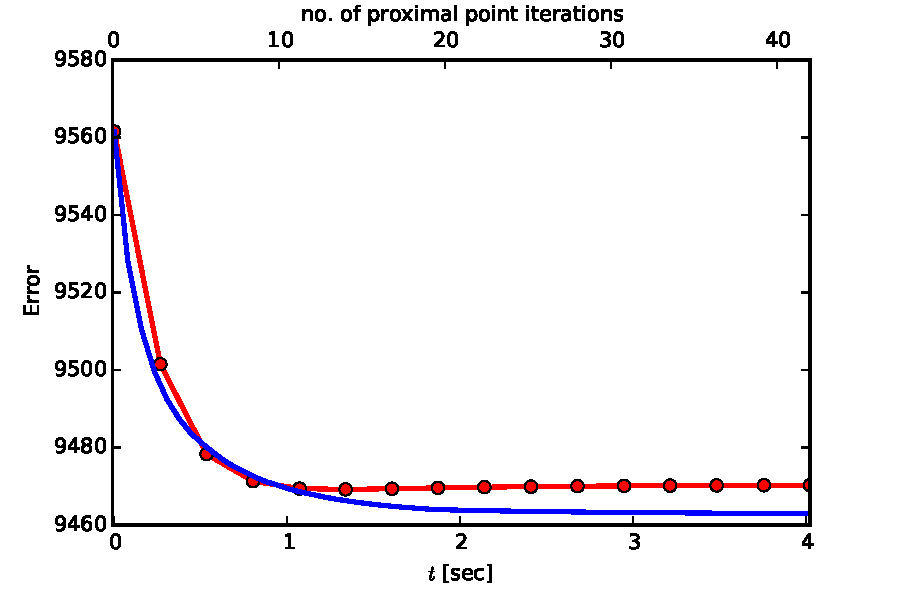
\includegraphics[width=0.5\linewidth]{./figures/experiments/SON_30x30_Err.pdf}
    }\\
    \subfloat[][$SO(3)$  (100$\times$100) - Functional]{
	\label{fig:comparison_son100J}
	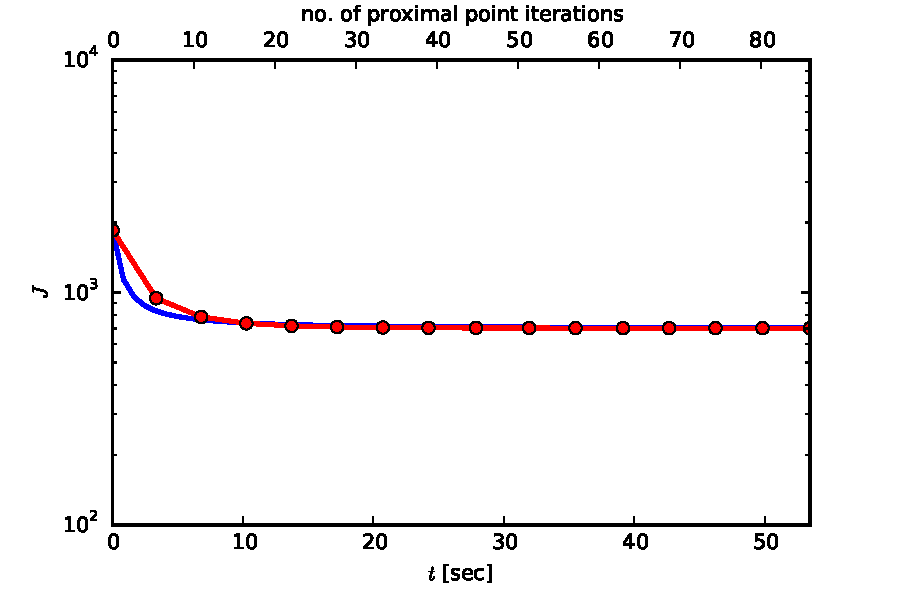
\includegraphics[width=0.5\linewidth]{./figures/experiments/SON_100x100_J.pdf}

    }
    \subfloat[][$SO(3)$ (100$\times$100 - Error]{
	\label{fig:comparison_son100E}
	\includegraphics[width=0.5\linewidth]{./figures/experiments/SON_100x100_Err.pdf}
    }\\
    \caption[Comparison IRLS \& PRPT for Euclidian $SO(3)$]{$SO(3)$: Comparison of functional value and errors for IRLS and PRPT minimizers.
	The red circles correspond to IRLS iterations while the line without any markers belongs to the proximal point iterations.
	\subref{fig:comparison_son30J} Functional values for synthetic 30$\times$30 $SO(3)$
	\subref{fig:comparison_son30E}  Errors relative to minimizer for synthetic 30$\times$30 $SO(3)$
	\subref{fig:comparison_son100J}  Functional values for synthetic 100$\times$100 $SO(3)$
	\subref{fig:comparison_son100E}  Errors relative to minimizer synthetic 100$\times$100 $SO(3)$
	\label{fig:comparison_son}
    }
\end{figure}

For $SO(3)$, shown in \label{fig:comparison_son}, the difference again becomes much smaller, with both plots being very close and coinciding already after the second iteration. 
Next, in the case of $SPD(3)$, shown in \label{fig:comparison_spd}, IRLS falls back to the niveau of $S^2$. One reason for that might the particularly complicated form of the second
derivative of the square distance function. This could be eventually optimized by improving the implementation of the Fr\'{e}chet derivative. At this time it is based on
the computation of a complex Schur decomposition which then, in turn, needs complex arithmetic. Switching to a block-based, but real Schur decomposition might provide an additional speed-up.

\begin{figure}[h!]
    \centering
    \subfloat[][$SPD(3)$ (30$\times$30) - Functional]{
	\label{fig:comparison_spd30J}
	\includegraphics[width=0.5\linewidth]{./figures/experiments/SPD_30x30_J.pdf}
    }
    \subfloat[][$SPD(3)$ (30$\times$30) - Error]{
	\label{fig:comparison_spd30E}
	\includegraphics[width=0.5\linewidth]{./figures/experiments/SPD_30x30_Err.pdf}
    }\\
    \caption[Comparison IRLS \& PRPT for Euclidian $SPD(3)$]{$SPD(3)$: Comparison of functional value and errors for IRLS and PRPT minimizers.
	The red circles correspond to IRLS iterations while the line without any markers belongs to the proximal point iterations.
	\subref{fig:comparison_spd30J} Functional values for synthetic 30$\times$30 $SPD(3)$ image
	\subref{fig:comparison_spd30E}  Error relative to minimizer for synthetic 30$\times$30 $SPD(3)$ image
	\label{fig:comparison_spd}
    }
\end{figure}


% section Comparison IRLS and Proximal Point minimizers (end)
\FloatBarrier
\section{Sensitivity to variations of the original data} % (fold)
\label{sec:Sensitivity}
%In section \ref{sub:Volume images} it was already mentioned that the computational and memory requirements become very demanding for increasing pixel numbers.
%If $N=XYZ$ denotes the number of pixels in the picture than the the number of non-zero entries in the Hessian is still $\mathcal{O}(N)$\\
In this section we perform a numerical experiment to see how changes of the noisy original picture influence the global solution found by the IRLS algorithm.
For that purpose we consider only the Brightness part of the Lena picture. In this grayscale image we pick a single non-zero pixel far enough in the inside of
the picture and set this pixel to zero, i.e. black color. This leads to two different original pictures
\begin{align}
    u_0,\hat{u}_0:\Omega &\to\mathbb{R}\\
    (\hat{u}_0)_{ij}&=\begin{cases}
	0, & \text{ if } i=i_0:=100,j=j_0:=10\\
	(u_0)_{ij}, &\text{else}
    \end{cases}.
\end{align}

Then for the original $u_0$ and the modified image $\hat{u}_0$ an IRLS minimization with $\lambda=0.1$, 5 iterations and one Newton step per reweighting is
performed to compare the two the solutions $u$ and $\hat{u}$. We take the absolute differences $e_{ij}=|u_{ij}-\hat{u}_{ij}|$ between the solutions
which leads to the error cone shown in Figure \ref{fig:experiment_sensitivity}\label{fig:experiment_sensitivity_plot}. This already suggests that the
error caused by changing the orginal data decays exponentially with distance $r=\sqrt{(i-i_0)^{2}+(j-j_0)^{2}}$.\\

After fitting a cone to the data, which is shown in \ref{fig:experiment_sensitivity}\label{fig:experiment_sensitivity_fit}
one finds that the aperture half-angle corresponds to a slope of $c=1.XXX$ such that the error will decay as
\begin{equation}
    e_{ij}=e^{-cr}.
\end{equation}

\begin{figure}[h!]
    \centering
    \subfloat[][Error cone]{
	\label{fig:experiment_sensitivity_plot}
	\includegraphics[width=0.4\linewidth]{./figures/experiments/cone.pdf}
    }
    \subfloat[][Fitted cone]{
	\label{fig:experiment_sensitivity_fit}
	\includegraphics[width=0.4\linewidth]{./figures/experiments/fitted_cone.pdf}
    }\\
    \caption[Sensitivity to variation]{Sensitivity to change in original data
	\subref{fig:experiment_sensitivity_plot} Logarithmic plot of absolut differences $e_{ij}=|u_{ij}-\hat{u}_{ij}|$
	\subref{fig:experiment_sensitivity_fit} Cone fitted to the data, resulting in aperture half-angle of $\alpha=XXX$
	\label{fig:experiment_sensitivity}
    }
\end{figure}

The most important conclusion one can draw from this is that a pixel in the global minimizer depends practically only on a local neighborhood of that pixel
in the original picture, not on pixels far away from that neighborhood. We will discuss possible applications of this in section \label{sec:Recursivecomputationonsubdomains}.\\

Of course these findings should be verified analytically by providing sufficiently precise error bounds, which is, however, unfortunately out of the scope of this work.

% section Sensitivity to variations of the starting value (end)

\end{chapter}
